\documentclass[14pt,aspectratio=169]{beamer}
%%%%%%%%%%%%%%%%%%%%%%%%%%%%%%%%%%%%%%%%%%%%%%%%%%%%%%%%%%%%%
% Meta informations:
\newcommand{\trauthor}{Felix Beese, Jens Lohmann}
\newcommand{\trtype}{}
\newcommand{\trcourse}{Bio-Inspired Artificial Intelligence}
\newcommand{\trtitle}{Discrete Tree-seed Algorithm for Solving Symmetric Traveling Salesman Problem}
\newcommand{\trmatrikelnummer}{6945957, 7326088}
\newcommand{\tremail}{hansen@informatik.uni-hamburg.de}
\newcommand{\trinstitute}{Dept. Informatik -- Knowledge Technology, WTM}
\newcommand{\trwebsiteordate}{{http://www.informatik.uni-hamburg.de/WTM/}}

%%%%%%%%%%%%%%%%%%%%%%%%%%%%%%%%%%%%%%%%%%%%%%%%%%%%%%%%%%%%%
% Languages:

% Falls die Ausarbeitung in Deutsch erfolgt:
% \usepackage[german]{babel}
% \usepackage[T1]{fontenc}
% \usepackage[latin1]{inputenc}
% \usepackage[latin9]{inputenc}	 				
% \selectlanguage{german}

% If the thesis is written in English:
\usepackage[english]{babel} 						
\selectlanguage{english}

%%%%%%%%%%%%%%%%%%%%%%%%%%%%%%%%%%%%%%%%%%%%%%%%%%%%%%%%%%%%%
% Bind packages:
\usepackage{beamerthemesplit}
\usetheme{Boadilla}
%\usetheme{Copenhagen}
%\usetheme{Darmstadt}
%\usetheme{Frankfurt}
%\usetheme{Ilmenau}
%\usetheme{JuanLesPins}
%\usetheme{Madrid}
%\usetheme{Warsaw }
%\usecolortheme{dolphin}
%\setbeamertemplate{sections/subsections in toc}[sections numbered]
%\beamertemplatenavigationsymbolsempty
%\setbeamertemplate{headline}[default] 	% deaktiviert die Kopfzeile
\setbeamertemplate{navigation symbols}{}% deaktiviert Navigationssymbole
%\useinnertheme{rounded}

\usepackage{acronym}                    % Acronyms
\usepackage[ruled,vlined]{algorithm2e}		% Algorithms and Pseudocode
%\usepackage{algorithmic}								% Algorithms and Pseudocode
%\usepackage{algorithm}									% Algorithms and Pseudocode
\usepackage{amsfonts}                   % AMS Math Packet (Fonts)
\usepackage{amsmath}                    % AMS Math Packet
\usepackage{amssymb}                    % Additional mathematical symbols
\usepackage{amsthm}
\usepackage{color}                      % Enables defining of colors via \definecolor
\usepackage{fancybox}                   % Gleichungen einrahmen
\usepackage{fancyhdr}										% Paket zur schickeren der Gestaltung der 
\usepackage{graphicx}                   % Inclusion of graphics
%\usepackage{latexsym}                  % Special symbols
\usepackage{longtable}									% Allow tables over several parges
\usepackage{listings}                   % Nicer source code listings
\usepackage{lmodern}
\usepackage{multicol}										% Content of a table over several columns
\usepackage{multirow}										% Content of a table over several rows
\usepackage{rotating}										% Alows to rotate text and objects
\usepackage[section]{placeins}          % Ermoeglich \Floatbarrier fuer Gleitobj. 
\usepackage[hang]{subfigure}            % Allows to use multiple (partial) figures in a fig
%\usepackage[font=footnotesize,labelfont=rm]{subfig}	% Pictures in a floating environment
\usepackage{tabularx}										% Tables with fixed width but variable rows
\usepackage{url,xspace,boxedminipage}   % Accurate display of URLs
\usepackage{tikz}
\usetikzlibrary{positioning}

\definecolor{uhhRed}{RGB}{226,0,26}     % Official Uni Hamburg Red
\definecolor{uhhGrey}{RGB}{136,136,136} % Official Uni Hamburg Grey
\definecolor{uhhLightGrey}{RGB}{220, 220, 220}
\setbeamertemplate{itemize items}[ball]
\setbeamercolor{title}{fg=uhhRed,bg=white}
\setbeamercolor{title in head/foot}{bg=uhhRed}
\setbeamercolor{block title}{bg=uhhGrey,fg=white}
\setbeamercolor{block body}{bg=uhhLightGrey,fg=black}
\setbeamercolor{section in head/foot}{bg=black}
\setbeamercolor{frametitle}{bg=white,fg=uhhRed}
\setbeamercolor{author in head/foot}{bg=black,fg=white}
\setbeamercolor{author in footline}{bg=white,fg=black}
\setbeamercolor*{item}{fg=uhhRed}
\setbeamercolor*{section in toc}{fg=black}
\setbeamercolor*{separation line}{bg=black}
\setbeamerfont*{author in footline}{size=\scriptsize,series=\mdseries}
\setbeamerfont*{institute}{size=\footnotesize}

\newcommand{\opticalseperator}{0.0025\paperwidth}

\institute{Universit\"at Hamburg\\\trinstitute}
\title{\trtitle}
\subtitle{\trtype}
\author{\trauthor}
\date{}
\logo{}

%%%%%%%%%%%%%%%%%%%%%%%%%%%%%%%%%%%%%%%%%%%%%%%%%%%%%%%%%%%%%
% Configurationen:
%\hypersetup{pdfpagemode=FullScreen}

\hyphenation{whe-ther} 									% Manually use: "\-" in a word: Staats\-ver\-trag

%\lstloadlanguages{C}                   % Set the default language for listings
\DeclareGraphicsExtensions{.pdf,.svg,.jpg,.png,.eps} % first try pdf, then eps, png and jpg
\graphicspath{{./src/}} 								% Path to a folder where all pictures are located

%%%%%%%%%%%%%%%%%%%%%%%%%%%%
% Costom Definitions:
\setbeamertemplate{title page}
{
  \vbox{}
	\vspace{0.4cm}
  \begin{centering}
    \begin{beamercolorbox}[sep=8pt,center,colsep=-4bp]{title}
      \usebeamerfont{title}\inserttitle\par%
    \end{beamercolorbox}%
    \begin{beamercolorbox}[sep=8pt,center,colsep=-4bp,rounded=true,shadow=true]{author}
      \usebeamerfont{author}\insertauthor \\ \insertinstitute
    \end{beamercolorbox}

	  \vfill
	  \begin{beamercolorbox}[ht=8ex,center]{}
		  
\includegraphics[width=0.16\paperwidth]{wtmIcon.pdf}
	  \end{beamercolorbox}%
    \begin{beamercolorbox}[sep=8pt,center,colsep=-4bp,rounded=true,shadow=true]{institute}
      \usebeamerfont{institute}\trwebsiteordate
    \end{beamercolorbox}
  \end{centering}
}

\setbeamertemplate{frametitle}
{
\begin{beamercolorbox}[wd=\paperwidth,ht=3.8ex,dp=1.2ex,leftskip=0pt,rightskip=4.0ex]{frametitle}%
		\usebeamerfont*{frametitle}\centerline{\insertframetitle}
	\end{beamercolorbox}
	\vspace{0.0cm}
}

\setbeamertemplate{footline}
{
	\hspace{15cm}
	\usebeamerfont*{author in footline}\insertframenumber{}
	\vspace{0.55cm}
}
\renewcommand{\footnotesize}{\fontsize{12.4pt}{12.4pt}\selectfont}
\renewcommand{\small}{\fontsize{13.8pt}{13.8pt}\selectfont}
\renewcommand{\normalsize}{\fontsize{15.15pt}{15.15pt}\selectfont}
\renewcommand{\large}{\fontsize{17.7pt}{17.7pt}\selectfont}
\renewcommand{\Large}{\fontsize{21.3pt}{21.3pt}\selectfont}

%%%%%%%%%%%%%%%%%%%%%%%%%%%%
% Additional 'theorem' and 'definition' blocks:
\newtheorem{axiom}{Axiom}[section] 	
%\newtheorem{axiom}{Fakt}[section]			% Wenn in Deutsch geschrieben wird.
%Usage:%\begin{axiom}[optional description]%Main part%\end{fakt}

%Additional types of axioms:
\newtheorem{observation}[axiom]{Observation}

%Additional types of definitions:
\theoremstyle{remark}
%\newtheorem{remark}[section]{Bemerkung} % Wenn in Deutsch geschrieben wird.
\newtheorem{remark}[section]{Remark} 

%%%%%%%%%%%%%%%%%%%%%%%%%%%%
% Provides TODOs within the margin:
\newcommand{\TODO}[1]{\marginpar{\emph{\small{{\bf TODO: } #1}}}}

%%%%%%%%%%%%%%%%%%%%%%%%%%%%
% Abbreviations and mathematical symbols
\newcommand{\modd}{\text{ mod }}
\newcommand{\RS}{\mathbb{R}}
\newcommand{\NS}{\mathbb{N}}
\newcommand{\ZS}{\mathbb{Z}}
\newcommand{\dnormal}{\mathit{N}}
\newcommand{\duniform}{\mathit{U}}

\newcommand{\erdos}{Erd\H{o}s}
\newcommand{\renyi}{-R\'{e}nyi}

%%%%%%%%%%%%%%%%%%%%%%%%%%%%
% Display of TOCs:
\AtBeginSection[]
{
	\setcounter{tocdepth}{2}  
	\frame
	{
	  \frametitle{Outline}
		\tableofcontents[currentsection]
	}
}
 
%%%%%%%%%%%%%%%%%%%%%%%%%%%%%%%%%%%%%%%%%%%%%%%%%%%%%%%%%%%%%
% Document:
\begin{document}
\renewcommand{\arraystretch}{1.2}

\begin{frame}[plain] % plain => kein Rahmen
  \titlepage
\end{frame}
%\setcounter{framenumber}{0}

\frame{
	\frametitle{Outline}
	\tableofcontents
}

%%%%%%%%%%%%%%
% Your Content

\section{Motivation and Question}

\frame[t]{
	\frametitle{Motivation and Question}
	\begin{itemize}
  		\item Discrete Tree-Seed Algorithm uses concept of trees and seeds
		\item Genetic Algorithms use concept of evolution
		\item Seems like they work in a quite similar way
		\begin{itemize}
			\item Is the DTSA a Genetic algorithm in disguise?
			\item What are the main differences?
		\end{itemize}
		\item Investigated by the Traveling Salesman Problem
	\end{itemize}
}

%%%%%%%%%%%%%%
\section{Basics and Definition}

\frame[t]{
	\frametitle{Traveling Salesman Problem}
	\begin{columns}[t]
		\begin{column}{.50\textwidth}
			\vspace{-0.5cm}
			\begin{itemize}
				\item Salesman has to visit many cities
				\item Wants to know the shortest tour
				\item \textbf{Goal:} find shortest Hamiltonian circle
				\item NP-hard problem
				\item Heuristic algorithms but also exact ones
			\end{itemize}
		\end{column}
		\begin{column}{.50\textwidth}
			\vspace{-1.25cm}
			\begin{figure}[ht]
				\centering		
				\includegraphics[scale=0.45]{./src/optimal_path_ch150}
				\caption{Example for a solved TSP.}
			\end{figure}
		\end{column}
	\end{columns}
}

\frame[t]{
	\frametitle{Discrete Tree-Seed Algorithm}
	\begin{columns}[t]
		\begin{column}{.5\textwidth}
			\begin{itemize}
				\item Iterative, heuristic algorithm
				\item Uses concept of trees and seeds (=possible solutions)
				\begin{itemize}
					\item get modified by operations
				\end{itemize}

				\item One tree as nearest neighbor tour
				\item Optimization of best result by 2-opt algorithm
			\end{itemize}
		\end{column}
		\begin{column}{.5\textwidth}
			\vspace{-1cm}
			\begin{figure}[ht]
				\centering		
				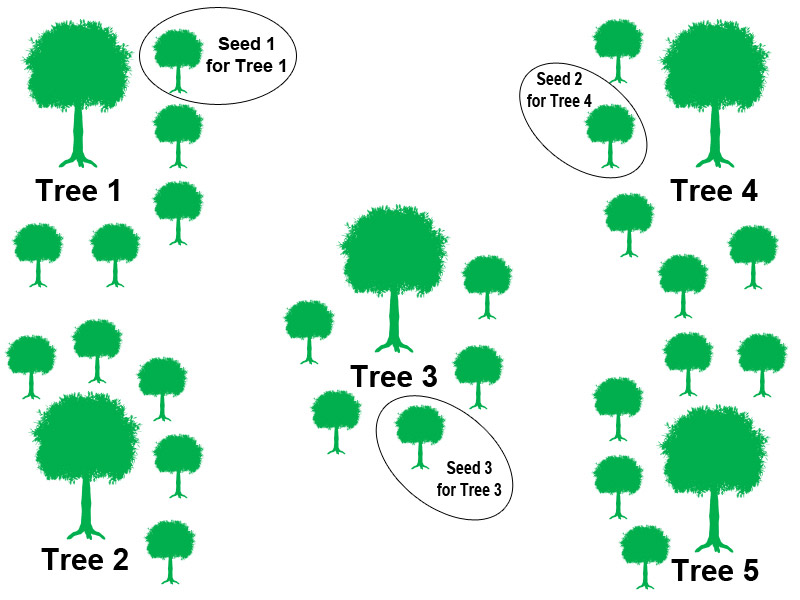
\includegraphics[scale=0.23]{./src/tree_seed}
				\caption{Figure by Kiran 2015} 
			\end{figure}
		\end{column}
	\end{columns}
}

\frame[t]{
	\frametitle{Operations}
	\begin{columns}
		\begin{column}{.55\textwidth}
			Operations used in algorithms:
			\begin{itemize}
				\item swap(i,j) = change cities at position i and j
				\item shift(i,j) = move path[i+1:j] one to the left and place overwritten city at j
				\item symmetry(i,j) = change direction of (sub)path[i:j]
			\end{itemize}
		\end{column}
		\begin{column}{.45\textwidth}
			\begin{figure}[ht]
				\centering		
				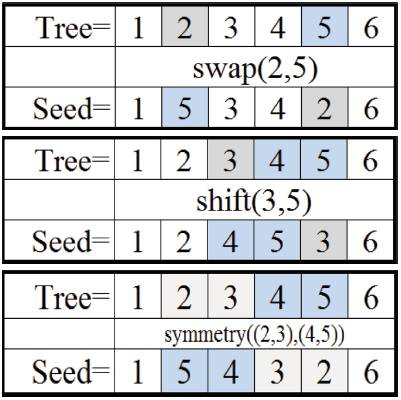
\includegraphics[scale=0.5]{./src/operations}
			\end{figure}
		\end{column}
	\end{columns}
}

\frame[t]{
	\frametitle{Genetic Algorithms}
	Genetic Algorithms are inspired by the concept of evolution
	\begin{itemize}
		\item Solutions represented as chromosomes (=linear representation)
		\item Working with generations (batches)
		\item Mutation and Crossover operations to create new solutions
		\item Selection step to choose the strongest/best solutions
	\end{itemize}
	\begin{figure}
		\begin{tikzpicture}[
			parent1/.style={rectangle, draw=blue!60, fill=blue!5, very thick, minimum size=5mm},
			parent2/.style={rectangle, draw=red!60, fill=red!5, very thick, minimum size=5mm},
			mutation/.style={rectangle, draw=green!60, fill=green!5, very thick, minimum size=7.63mm},
			description/.style={very thick, minimum size=5mm},
			]
			%Nodes
				\node[description]	(crossover)		at (1.8,1)	{Crossover};
				\node[description]	(mutation)		at (7.9,1)	{Mutation};
				\node[parent1]		(parent1)		at (0,0)			{7,5,11,9,3};
				\node[parent2]		(parent2)		at (0,-1)		{11,6,2,5,8};
				\node[parent1]		(child-1)		at (3.0,-0.5)	{7,5};
				\node[parent2]		(child-2)		at (4.26,-0.5)	{2,5,8};
				\node[parent1]		(mutant-1)		at (7,-0.5)		{7,5};
				\node[mutation]		(mutant-2)		at (7.93,-0.5)	{4};
				\node[parent2]		(mutant-3)		at (8.86,-0.5)	{5,8};

			%Lines
				\draw[very thick,->] (parent1.east) -- (child-1);
				\draw[very thick,->] (parent2.east) -- (child-1);
				\draw[very thick,->] (child-2) -- (mutant-1);
		\end{tikzpicture}
	\end{figure}
}

%%%%%%%%%%%%%%
\section{Approach}

\frame[t]{
	\frametitle{Proceeding}
	\begin{enumerate}
		\item Implemented two algorithms
		\begin{itemize}
			\item Discrete Tree-Seed Algorithm
			\item Genetic Algorithm
		\end{itemize}
		\item Each algorithm run 90 times
		\begin{itemize}
			\item Six problem instances were taken from tsplib95\\
			berlin52, st70, kroA100, eil101, ch150, tsp225
			%NOTES:
			% TSPlib95 is a Python library for handling TSPs and similar problems.
			% It offers read and write problems and paths, also optimal paths for the problems.
		\end{itemize}
		\item Compared the results
		\begin{itemize}
			\item By computing statistical metrics % like mean and standard deviation
			\item And using different visualization methods % Convergence over time, boxplots and the tours itself
			\item \textbf{Goal:} Finding similarities and differences of DTSA and GA
		\end{itemize}
	\end{enumerate}
}

\frame[t]{
	\frametitle{DTSA - Main Procedure}
	\begin{itemize}
		\item create $k-1$ random trees, one by NN-tour
		\item repeat until stopping criterion is met
			\begin{itemize}
				\item loop over all trees/paths (current tree)
				\begin{itemize}
					\item choose random to create 3 seeds by operations on best tree or current tree
					\item create 3 seeds by operations on random tree
					\item get best tree out of those 6+1 trees for next iteration
				\end{itemize}
				\item $k$ new trees were chosen
				\item check if stopping criterion is met
			\end{itemize}
		\item return overall best tree optimized by 2-opt
	\end{itemize}
}

\frame[t]{
	\frametitle{Genetic Algorithm - Main Procedure}
	GTSPA = \emph{Genetic Traveling Salesman Problem Algorithm}
	\begin{itemize}
		\item create $k-1$ random trees, one by NN-tour
		\item repeat until stopping criterion is met
			\begin{itemize}
				\item loop over all trees/paths (current tree)
				\begin{itemize}
					\item \colorbox{yellow}{create 3 seeds by operations on current tree}
				\end{itemize}
				\item \colorbox{yellow}{get best $k$ trees out of those $4 \cdot k$ trees for next iteration}
				\item $k$ new trees were chosen
				\item check if stopping criterion is met
			\end{itemize}
		\item return overall best tree optimized by 2-opt
	\end{itemize}
}

\frame[t]{
	\frametitle{Crossover for Trees}
	\begin{columns}[t]
	\begin{column}{.55\textwidth}
	\vspace{-0.25cm}
	\begin{itemize}
		\item Not working with paths every time
		\item Often gives a useless result
		\item Not needed for asexual reproduction
	\end{itemize}
	\begin{figure}
		\begin{tikzpicture}[
			parent1/.style={rectangle, draw=blue!60, fill=blue!5, very thick, minimum size=5mm},
			parent2/.style={rectangle, draw=red!60, fill=red!5, very thick, minimum size=5mm},
			]
			%Nodes
				\node[parent1]		(parent1-1)		at (0,0)			{1,2,3};
				\node[parent1]		(parent1-2)		at (1.2,0)		{4,5};
				\node[parent2]		(parent2-1)		at (0,-1)		{1,4,5};
				\node[parent2]		(parent2-2)		at (1.2,-1)		{3,2};
				\node[parent1]		(child-1)		at (5,-0.5)		{1,2,3};
				\node[parent2]		(child-2)		at (6.26,-0.5)	{3,2};

			%Lines
				\draw[very thick,->] (parent1-2.east) -- (child-1);
				\draw[very thick,->] (parent2-2.east) -- (child-1);
		\end{tikzpicture}
	\end{figure}
	\end{column}
	\begin{column}{.45\textwidth}
	\vspace{-1cm}
	\begin{figure}
		\begin{tikzpicture}[
			parent1/.style={rectangle, draw=blue!60, fill=blue!5, very thick, minimum size=5mm},
			parent2/.style={rectangle, draw=red!60, fill=red!5, very thick, minimum size=5mm},
			]
			%Nodes
				% blue nodes
				\node[]		(blue1)		at (0,2)		{1};
				\node[]		(blue2)		at (2,2)		{2};
				\node[]		(blue3)		at (1,1)		{3};
				\node[]		(blue4)		at (0,0)		{4};
				\node[]		(blue5)		at (2,0)		{5};
				% red nodes
				\node[]		(red1)		at (4,2)		{1};
				\node[]		(red2)		at (6,2)		{2};
				\node[]		(red3)		at (5,1)		{3};
				\node[]		(red4)		at (4,0)		{4};
				\node[]		(red5)		at (6,0)		{5};
				% child nodes
				\node[]		(child1)		at (2,-2)		{1};
				\node[]		(child2)		at (4,-2)		{2};
				\node[]		(child3)		at (3,-3)		{3};
				\node[]		(child4)		at (2,-4)		{4};
				\node[]		(child5)		at (4,-4)		{5};
				%ghost nodes for parent arrows
				\node[]		(parent1)		at (1,0)		{};
				\node[]		(parent2)		at (5,0)		{};
				\node[]		(child)			at (3,-2)		{};

			%Lines
				% blue graph
				\draw[very thick, color=blue] (blue1) -- (blue2);
				\draw[very thick, color=blue] (blue2) -- (blue3);
				\draw[very thick, color=blue] (blue3) -- (blue4);
				\draw[very thick, color=blue] (blue4) -- (blue5);
				% red graph
				\draw[very thick, color=red] (red1) -- (red4);
				\draw[very thick, color=red] (red4) -- (red5);
				\draw[very thick, color=red] (red5) -- (red3);
				\draw[very thick, color=red] (red3) -- (red2);
				% child graph
				\draw[very thick, color=purple!60] (child1) -- (child2);
				\draw[very thick, color=purple!60] (child2.west) .. controls +(left:3mm) and +(up:3mm) .. (child3.north);
				\draw[very thick, color=purple!60] (child3.west) .. controls +(left:7mm) and +(down:7mm) .. (child3.south);
				\draw[very thick, color=purple!60] (child3.east) .. controls +(right:3mm) and +(down:3mm) .. (child2.south);
				% arrows
				\draw[very thick, ->] (parent1) -- (child);
				\draw[very thick, ->] (parent2) -- (child);
		\end{tikzpicture}
	\end{figure}
	\end{column}
	\end{columns}
}

\frame[t]{
	\frametitle{Genetic Algorithm - why three versions?}
	\begin{itemize}
	\item Three different versions were tested
	\item They differ in their order of mutation and selection
	\begin{itemize}
		\item GTSPA-SM
		\item GTSPA-MS
		\item GTSPA-SMS
	\end{itemize}
	\item The same effects could be achieved by using different\\ population sizes instead
	\end{itemize}	
}

%%%%%%%%%%%%%%
\section{Results}

\frame[t]{
	\frametitle{Path length over steps}
	\begin{columns}
		\begin{column}{.50\textwidth}
			\vspace{-0.75cm}
			\begin{figure}[ht]
				\centering		
				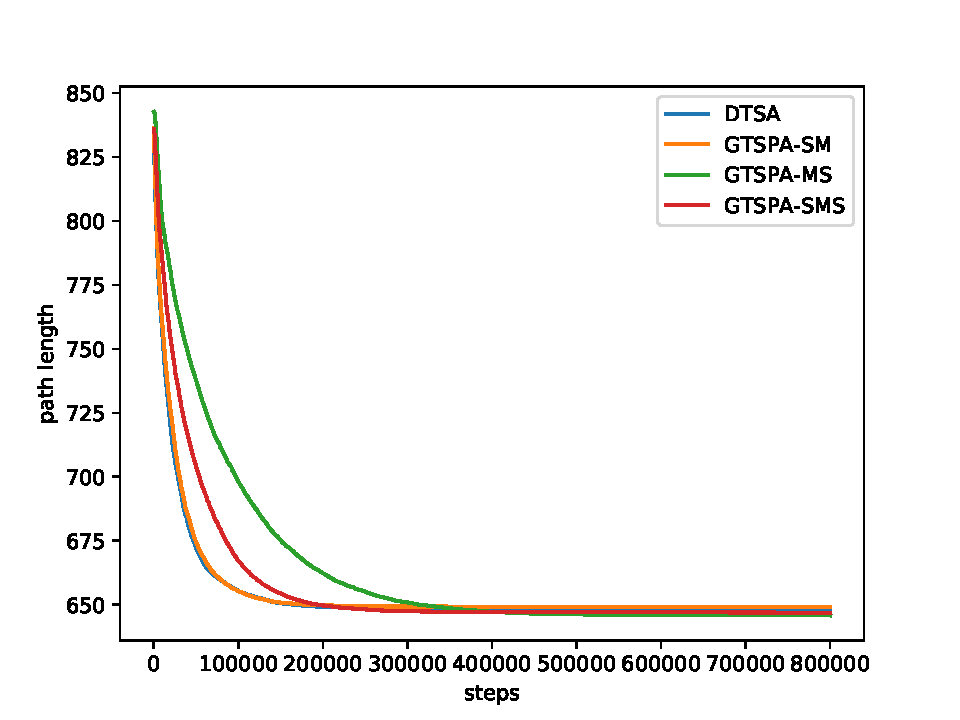
\includegraphics[scale=.45]{../Implementation/gen/mean_convergence_eil101}
				\caption{eil101}
			\end{figure}
		\end{column}
		\begin{column}{.50\textwidth}
			\vspace{-0.75cm}
			\begin{figure}[ht]
				\centering		
				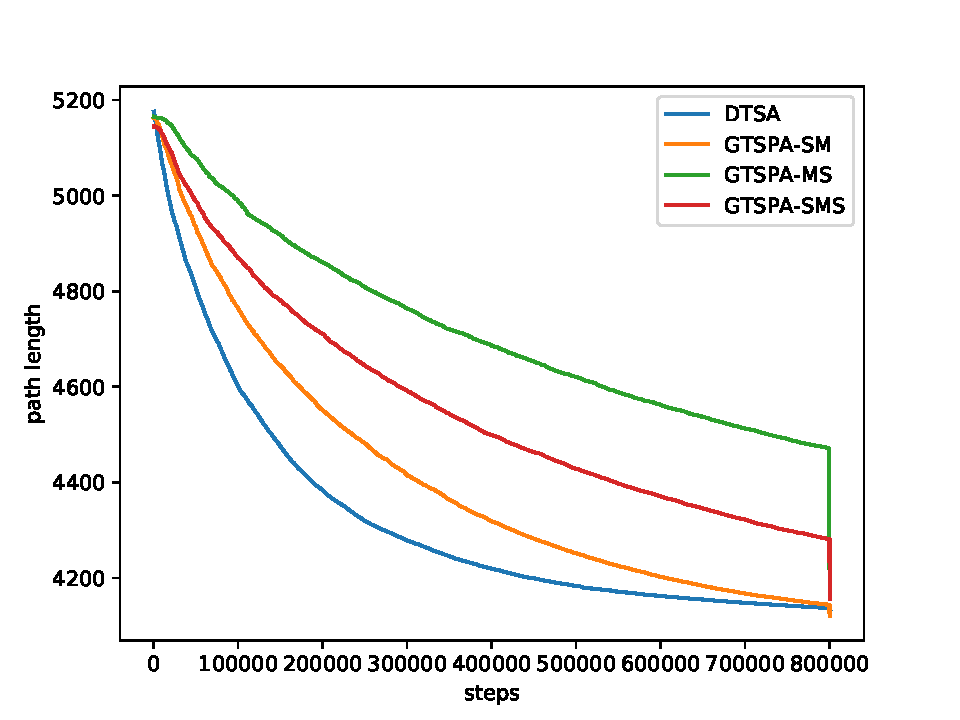
\includegraphics[scale=.45]{../Implementation/gen/mean_convergence_tsp225}
				\caption{tsp225}
			\end{figure}
		\end{column}
	\end{columns}
}

%TODO not show this slide but keep as notes
%\frame[t]{
%	\frametitle{Convergence of path length over iterations}
%	What can be seen in the six plots
%	\begin{itemize}
%		\item DTSA converges the fastest for each problem
%		\item GTSPA-MS converges slowest
%		\item Sharp cut in tsp225 is because of 2-opt
%		\item More steps would probably not lead to a better result, because stuck in local minimum
%		\item Running time increases (quadratic) with size of problem
%	\end{itemize}
%}

%What I would include as results slide for all boxplots and tables
%berlin52 shows that alle give at least once optimal results and overall paths in DTSA are a little bit longer
%tsp225 shows that results of dtsa are little bit better with large problems, but only a little bit
\frame[t]{
	\frametitle{Final path lengths (berlin52 \& tsp225)}
	\vspace{-1cm}
	\begin{columns}
		\begin{column}{.50\textwidth}
			\begin{figure}[ht]
				\centering
				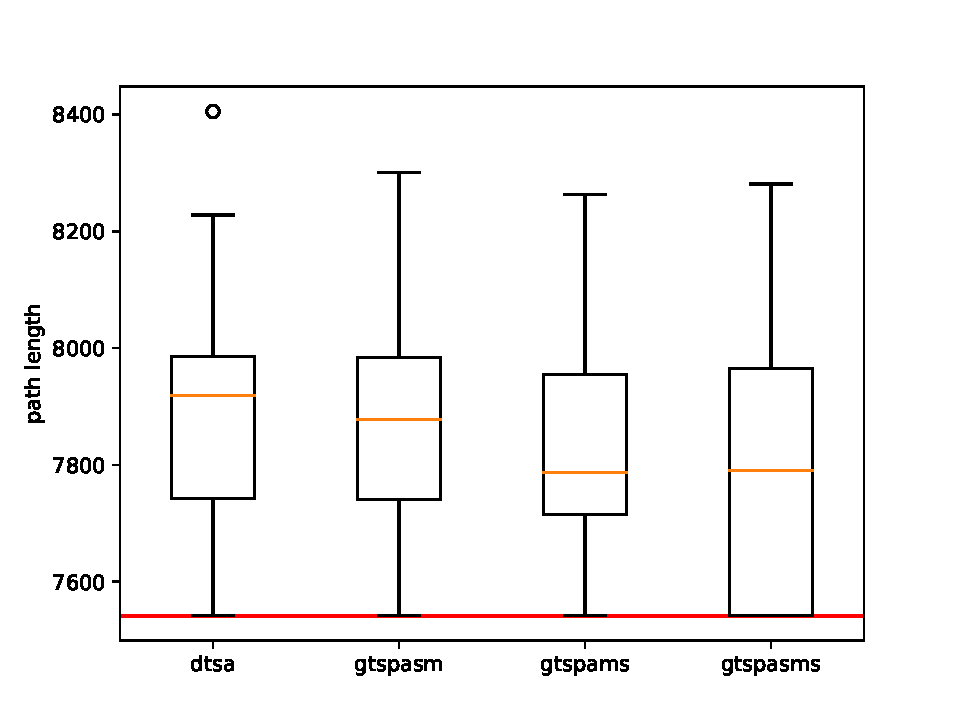
\includegraphics[width=\textwidth]{../Implementation/gen/boxplot_berlin52}
				\caption{berlin52}
			\end{figure}
		\end{column}
		
		\begin{column}{.50\textwidth}
			\begin{figure}[ht]
				\centering
				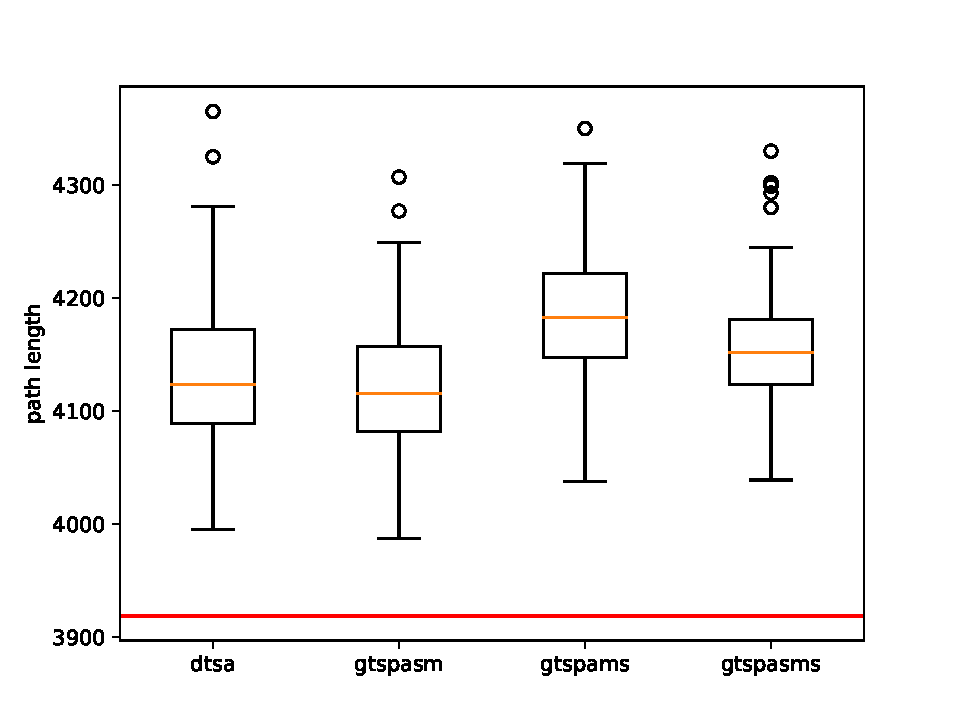
\includegraphics[width=\textwidth]{../Implementation/gen/boxplot_tsp225}
				\caption{tsp225}
			\end{figure}
		\end{column}
	\end{columns}
}

%TODO not show this slide but keep as notes
%\frame[t]{
%	\frametitle{Final tours}
%	\begin{itemize}
%		\item for berlin52 and kroA100 all algorithms give optimal solution at least once % This can easily seen in the table but also the boxplots show that they have the same best
%		\item for st70, eil101 and ch150 best paths have some small differences % Can be seen in boxplots
%		\item tsp225 has some interesting variation % The next slide shows this pretty well
%		\begin{itemize}
%			\item DTSA and GTSPA-SM: 'S' not visible (best path: 3995 \& 3987)
%			\item GTSPA-MS and GTSPA-SMS: 'S' can be noticed (best path: 4038 \& 4039)
%		\end{itemize}
%	\end{itemize}
%}

\frame[t]{
%	\frametitle{Final tours}
	\begin{columns}
		\begin{column}{0.32\textwidth}
			\centering
			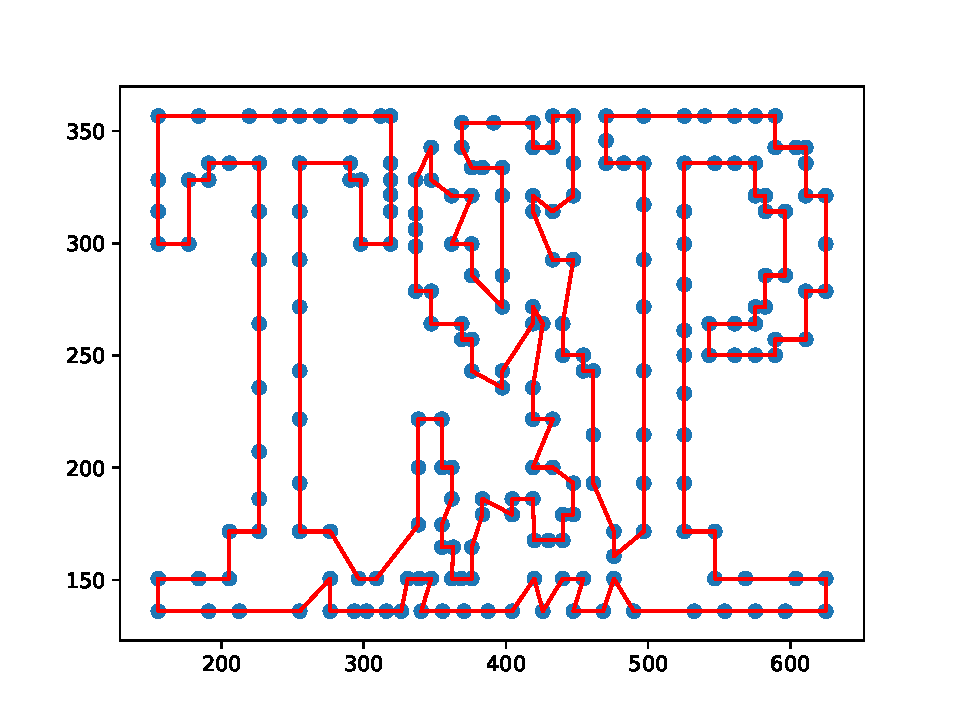
\includegraphics[width=\textwidth]{../Implementation/gen/best_path_dtsa_tsp225}\\
			{\color{blue}DTSA} (3995)
		\end{column}
		\begin{column}{0.32\textwidth}
			\centering
			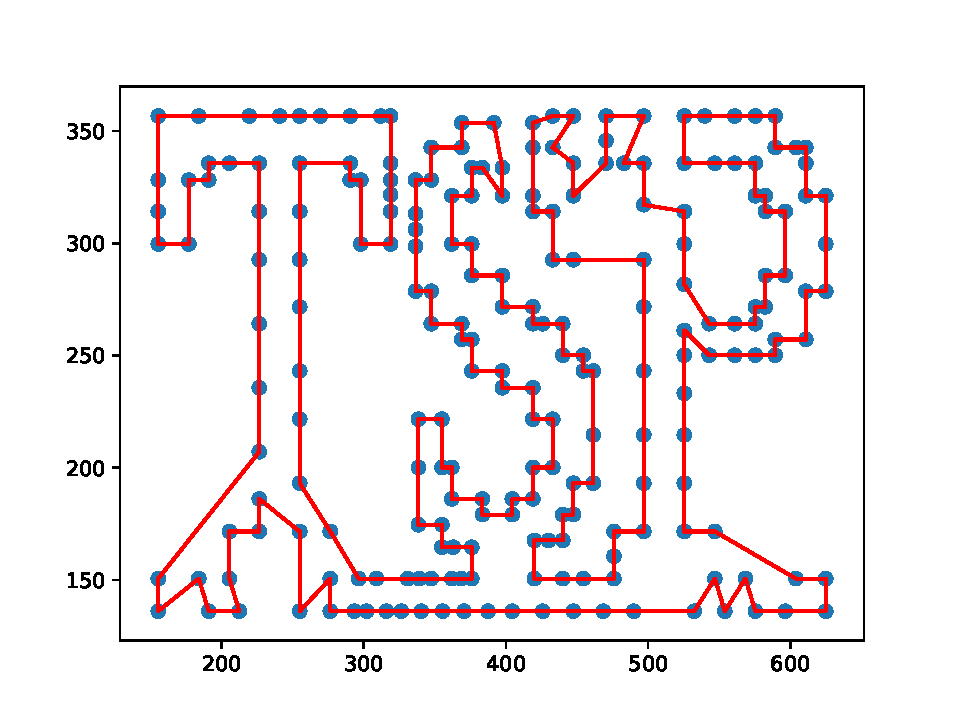
\includegraphics[width=\textwidth]{../Implementation/gen/best_path_gtspams_tsp225}\\
			{\color{blue}GTSPA-MS} (4038)
		\end{column}
		\begin{column}{0.32\textwidth}
			\centering
			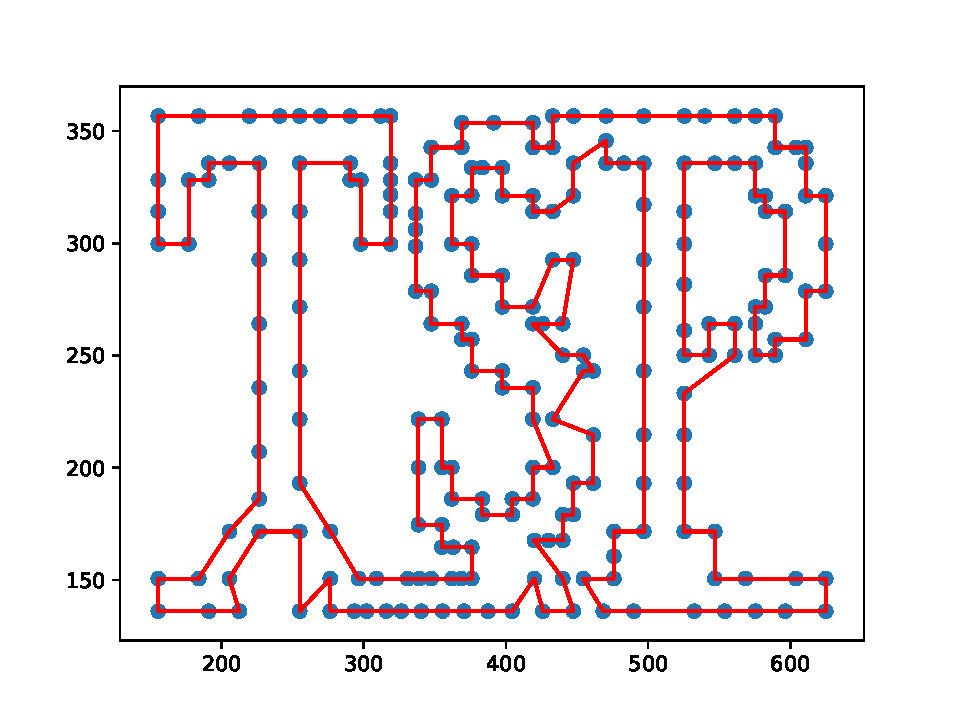
\includegraphics[width=\textwidth]{../Implementation/gen/best_path_gtspasms_tsp225}\\
			{\color{blue}GTSPA-SMS} (4039)
		\end{column}
	\end{columns}
	\begin{columns}
		\begin{column}{0.32\textwidth}
			\centering
			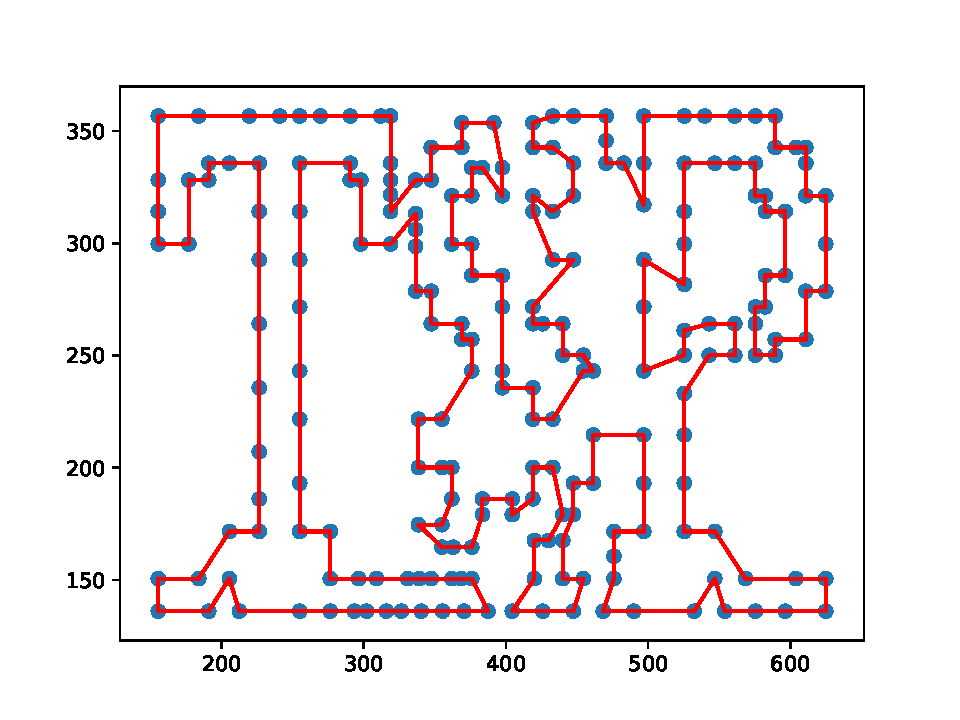
\includegraphics[width=\textwidth]{../Implementation/gen/best_path_gtspasm_tsp225}\\
			{\color{blue}GTSPA-SM} (3987)
		\end{column}
		\begin{column}{0.32\textwidth}
			\centering
			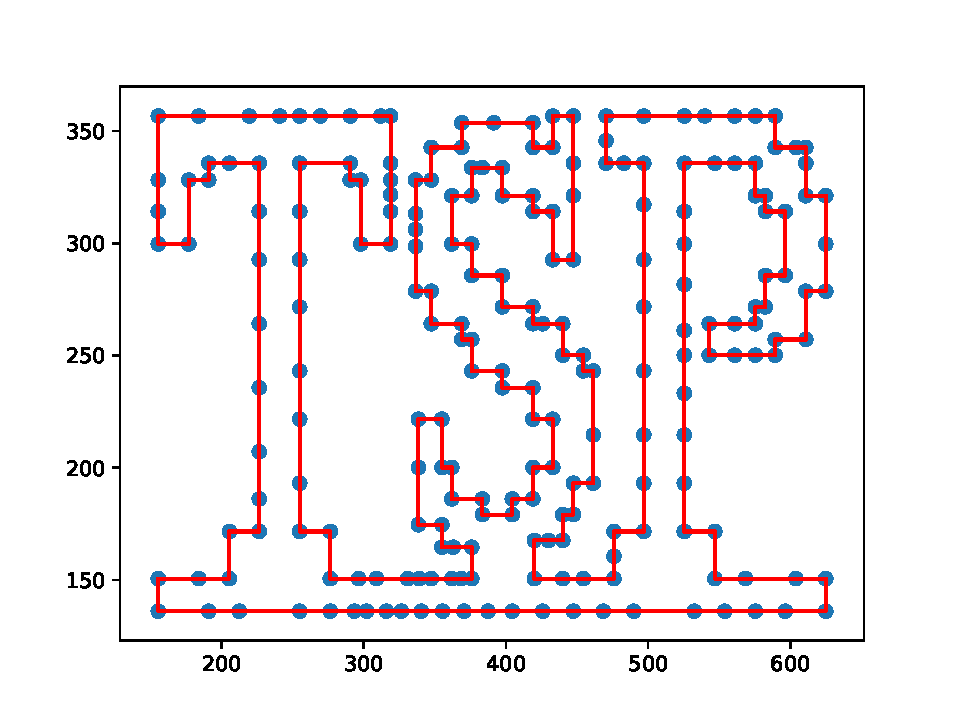
\includegraphics[width=\textwidth]{../Implementation/gen/optimal_path_tsp225}\\
			{\color{blue}Optimal} (3919)
		\end{column}
	\end{columns}
}

%%%%%%%%%%%%%%
\section{Conclusion}

\frame[t]{
	\frametitle{Comparison of DTSA and GA}
	\begin{columns}[t]
		\begin{column}{0.45\textwidth}
			{\color{blue} Similarities}:
			\begin{itemize}
				\item Concept of evolution with generations, mutations and, selection
				\item Same operations (swap, shift, symmetry)
				\item Give results of same magnitude
			\end{itemize}
		\end{column}
		\hspace{-0.05\textwidth}
		\begin{column}{0.45\textwidth}
			{\color{blue} Differences}:
			\begin{itemize}
				\item DTSA has different groups which evolve almost independently from each other
				% NOTES:
				% They still use the best or a random tree from so there is a mix between the solutions
				% Although we said crossover wasn't possible, in a way, this could be considered some kind of crossover where the genes of two different parent trees mix to create an offspring for the next generation
				\item DTSA converges a little bit faster
				\item DTSA gives a little worser overall results
			\end{itemize}
		\end{column}
	\end{columns}
}

\frame[t]{
	\frametitle{Open questions}
	What can be done now to explore further:
	\begin{itemize}
  		\item Test statistical parameters for significance (t-Test, ...)
		\item Try different parameters and investigate performance
		\item Implement a classical crossover operation
		\item Have a look at asymmetric TSP
	\end{itemize}
}

%%%%%%%%%%%%%%

\frame[c]{
	\frametitle{The End}
	\begin{center}
		\emph{"The DTSA is a Genetic Algorithm with small adjustments."}\\[3ex]
		Thank you for your attention.\\[1ex]
		Any question?\\[5ex]
	\end{center}
	\footnotesize
	Literature:
	\begin{itemize} %TODO add references for figures
		\item Ahmet Cevahir Cinar , Sedat Korkmaz, and Mustafa Servet Kiran. A discrete tree-seed algorithm for solving traveling salesman problem. \emph{In: Engineering Science and Technology}, 2020
	\end{itemize}
}

%%%%%%%%%%%%%
%  BONUS CONTENT
%%%%%%%%%%%%%

%TODO maybe show the table just for a short time but go straight to the boxplots which show the same information but visualized
\frame[t]{ 
	\frametitle{Final path lengths}
	\vspace{-1cm}
	\begin{table}[ht]
\begin{center}
\resizebox{\textwidth}{!}{%
\begin{tabular}{|c|c|c|c|c|c|c|}
	\hline
	dataset & algorithm & mean & std. dev. & best & worst & RE(\%)\\
	\hline
	\multirow{4}{*}{berlin52}		& DTSA & 7868.18 & 185.5 & \textbf{7542} & \textbf{8405} & 4.32\\
		& GTSPA-SM & 7867.68 & 193.33 & \textbf{7542} & 8301 & 4.32\\
		& GTSPA-MS & \textbf{7790.32} & 175.78 & \textbf{7542} & 8263 & 3.29\\
		& GTSPA-SMS & 7798.98 & 192.88 & \textbf{7542} & 8281 & 3.41\\
	\hline
	\multirow{4}{*}{st70}		& DTSA & 700.57 & 16.09 & 683 & 738 & 3.79\\
		& GTSPA-SM & 698.26 & 15.3 & \textbf{680} & \textbf{747} & 3.45\\
		& GTSPA-MS & \textbf{695.41} & 13.09 & 682 & 737 & 3.02\\
		& GTSPA-SMS & 695.47 & 12.2 & 682 & 741 & 3.03\\
	\hline
\end{tabular}}
\label{table:algo-stats}
\end{center}
\end{table}
}

\frame[t]{
	\frametitle{Final path lengths}
	\vspace{-1cm}
	\begin{table}[ht]
\begin{center}
\resizebox{\textwidth}{!}{%
\begin{tabular}{|c|c|c|c|c|c|c|}
	\hline
	dataset & algorithm & mean & std. dev. & best & worst & RE(\%)\\
	\hline
	\multirow{4}{*}{kroA100}		& DTSA & 21831.69 & 382.83 & \textbf{21282} & 23009 & 2.58\\
		& GTSPA-SM & 21754.38 & 355.07 & \textbf{21282}& 23136 & 2.22\\
		& GTSPA-MS & \textbf{21588.57} & 348.82 & \textbf{21282} & 23096 & 1.44\\
		& GTSPA-SMS & 21719.31 & 351.1 & \textbf{21282} & \textbf{23224} & 2.05\\
	\hline
	\multirow{4}{*}{eil101}		& DTSA & 647.76 & 8.45 & \textbf{629} & \textbf{671} & 2.98\\
		& GTSPA-SM & 648.99 & 8.66 & 630 & \textbf{671} & 3.18\\
		& GTSPA-MS & \textbf{645.92} & 7.22 & 631 & 665 & 2.69\\
		& GTSPA-SMS & 646.9 & 8.26 & 630 & 669 & 2.85\\
	\hline
\end{tabular}}
\label{table:algo-stats}
\end{center}
\end{table}
}

\frame[t]{
	\frametitle{Final path lengths}
	\vspace{-0.5cm}
	\begin{table}[ht]
\begin{center}
\resizebox{\textwidth}{!}{%
\begin{tabular}{|c|c|c|c|c|c|c|}
	\hline
	dataset & algorithm & mean & std. dev. & best & worst & RE(\%)\\
	\hline
	\multirow{4}{*}{ch150}		& DTSA & 6688.03 & 85.32 & 6549 & \textbf{6922} & 2.45\\
		& GTSPA-SM & 6683.87 & 88.31 & 6549 & 6898 & 2.39\\
		& GTSPA-MS & 6665.89 & 86.8 & 6552 & 6913 & 2.11\\
		& GTSPA-SMS & \textbf{6661.59} & 77.5 & \textbf{6544} & 6839 & 2.05\\
	\hline
	\multirow{4}{*}{tsp225}		& DTSA & 4132.73 & 64.11 & 3995 & \textbf{4365} & 5.45\\
		& GTSPA-SM & \textbf{4121.48} & 57.02 & \textbf{3987} & 4307 & 5.17\\
		& GTSPA-MS & 4188.68 & 55.87 & 4038 & 4350 & 6.88\\
		& GTSPA-SMS & 4156.21 & 54.31 & 4039 & 4330 & 6.05\\
	\hline
\end{tabular}}
\label{table:algo-stats}
\end{center}
\end{table}
}

\frame[t]{ 
	\frametitle{Final path lengths (berlin52 \& st70)}
	\vspace{-1cm}
	\begin{columns}
		\begin{column}{.50\textwidth}
			\begin{figure}[ht]
				\centering
				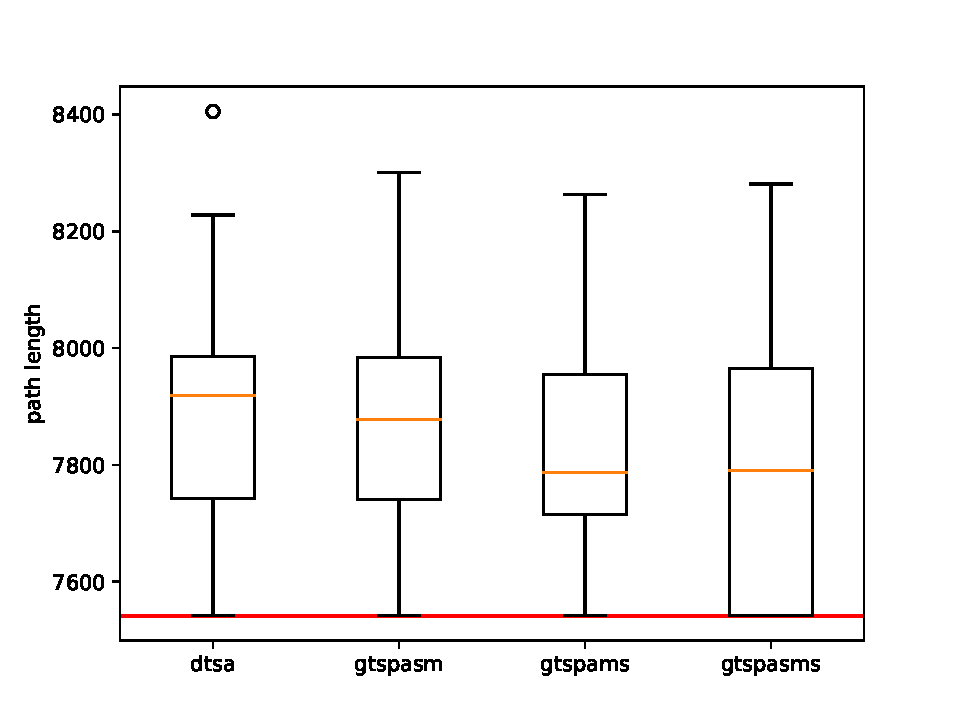
\includegraphics[width=\textwidth]{../Implementation/gen/boxplot_berlin52}
				\caption{berlin52}
			\end{figure}
		\end{column}
		
		\begin{column}{.50\textwidth}
			\begin{figure}[ht]
				\centering
				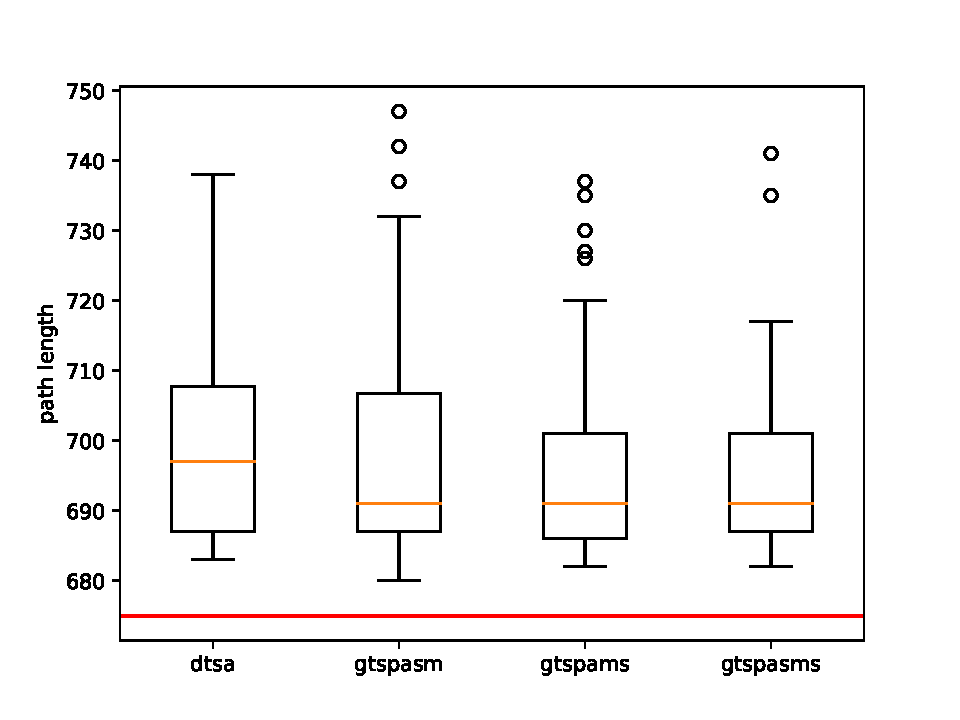
\includegraphics[width=\textwidth]{../Implementation/gen/boxplot_st70}
				\caption{st70}
			\end{figure}
		\end{column}
	\end{columns}
}

\frame[t]{
	\frametitle{Final path lengths (kroA100 \& eil101)}
	\vspace{-1cm}
	\begin{columns}
		\begin{column}{.50\textwidth}
			\begin{figure}[ht]
				\centering
				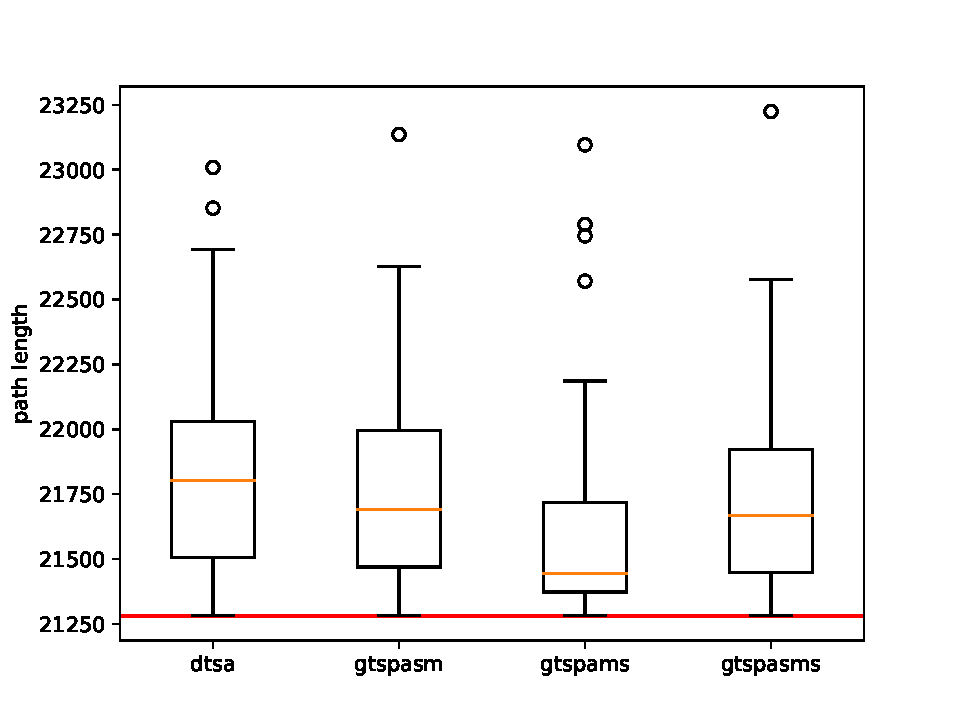
\includegraphics[width=\textwidth]{../Implementation/gen/boxplot_kroA100}
				\caption{kroA100}
			\end{figure}
		\end{column}
		
		\begin{column}{.50\textwidth}
			\begin{figure}[ht]
				\centering
				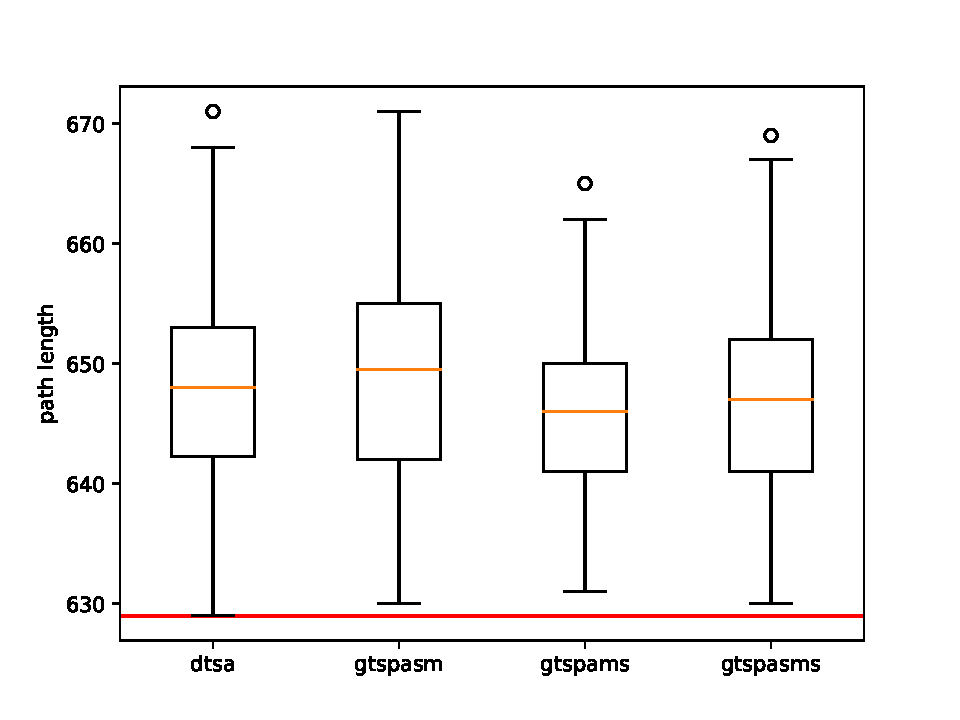
\includegraphics[width=\textwidth]{../Implementation/gen/boxplot_eil101}
				\caption{eil101}
			\end{figure}
		\end{column}
	\end{columns}
}

\frame[t]{
	\frametitle{Final path lengths (ch150 \& tsp225)}
	\vspace{-1cm}
	\begin{columns}
		\begin{column}{.50\textwidth}
			\begin{figure}[ht]
				\centering
				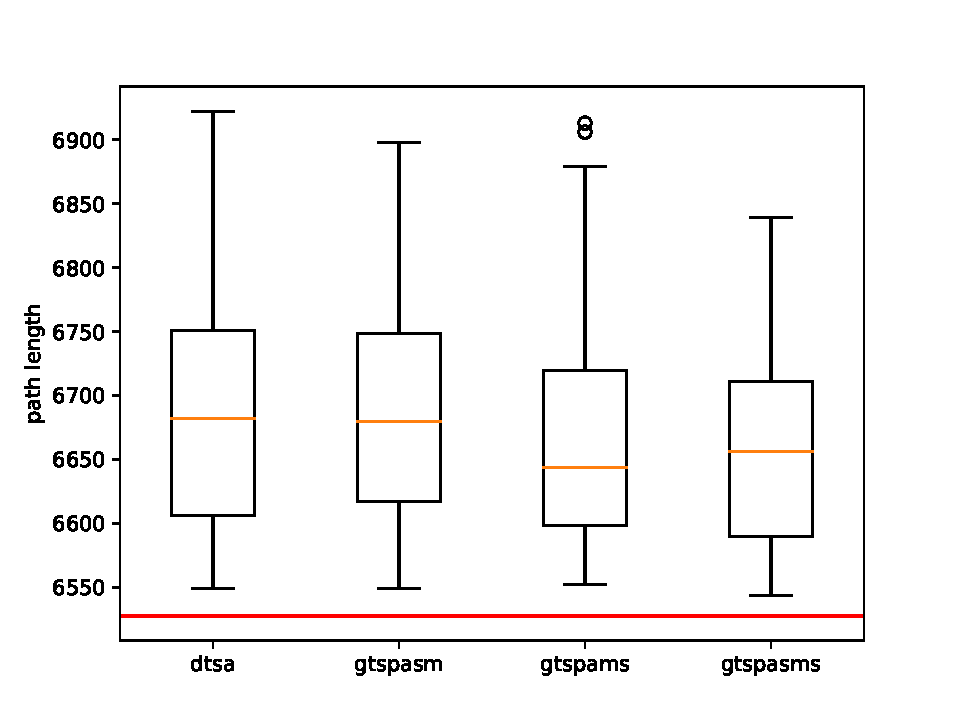
\includegraphics[width=\textwidth]{../Implementation/gen/boxplot_ch150}
				\caption{ch150}
			\end{figure}
		\end{column}
		
		\begin{column}{.50\textwidth}
			\begin{figure}[ht]
				\centering
				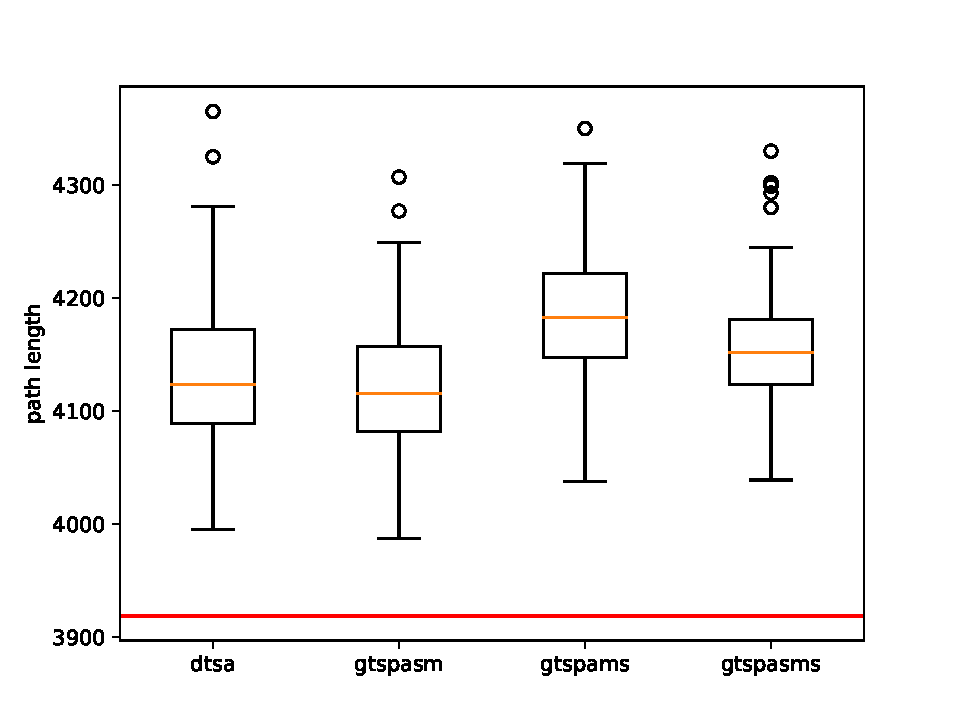
\includegraphics[width=\textwidth]{../Implementation/gen/boxplot_tsp225}
				\caption{tsp225}
			\end{figure}
		\end{column}
	\end{columns}
}

\frame[t]{
	\begin{columns}
		\begin{column}{0.32\textwidth}
			\centering
			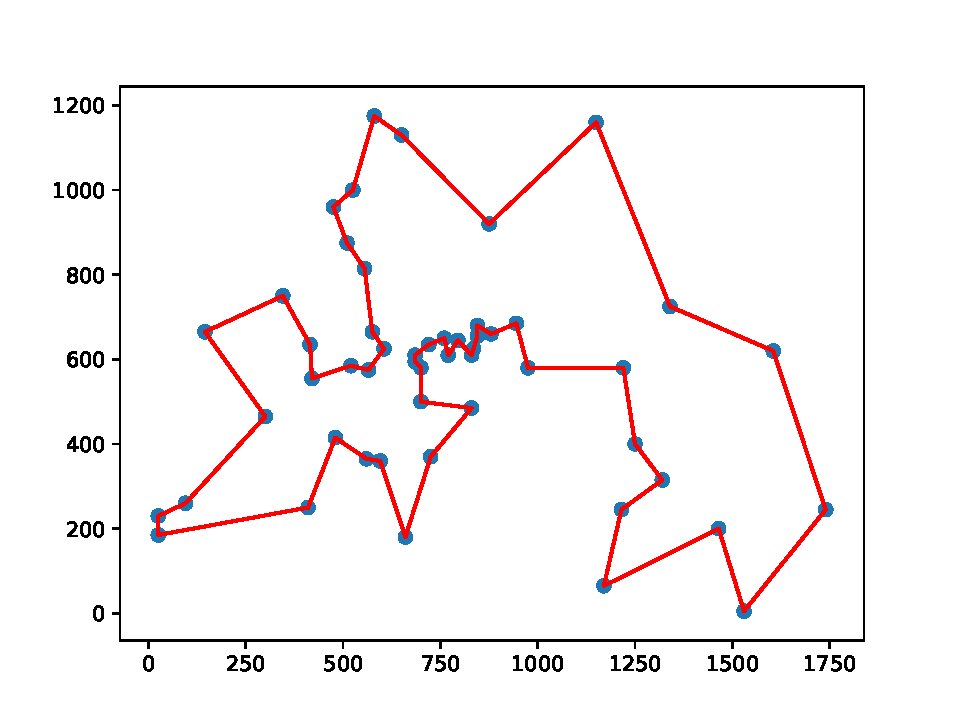
\includegraphics[width=\textwidth]{../Implementation/gen/best_path_dtsa_berlin52}\\
			{\color{blue}DTSA}
		\end{column}
		\begin{column}{0.32\textwidth}
			\centering
			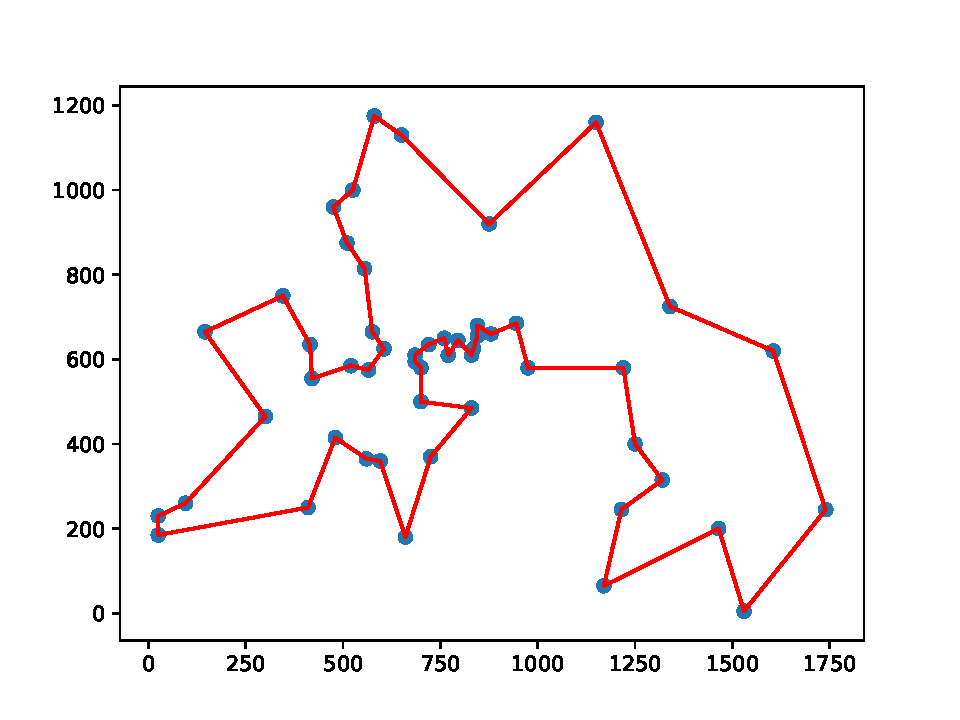
\includegraphics[width=\textwidth]{../Implementation/gen/best_path_gtspams_berlin52}\\
			{\color{blue}GTSPA-MS}
		\end{column}
		\begin{column}{0.32\textwidth}
			\centering
			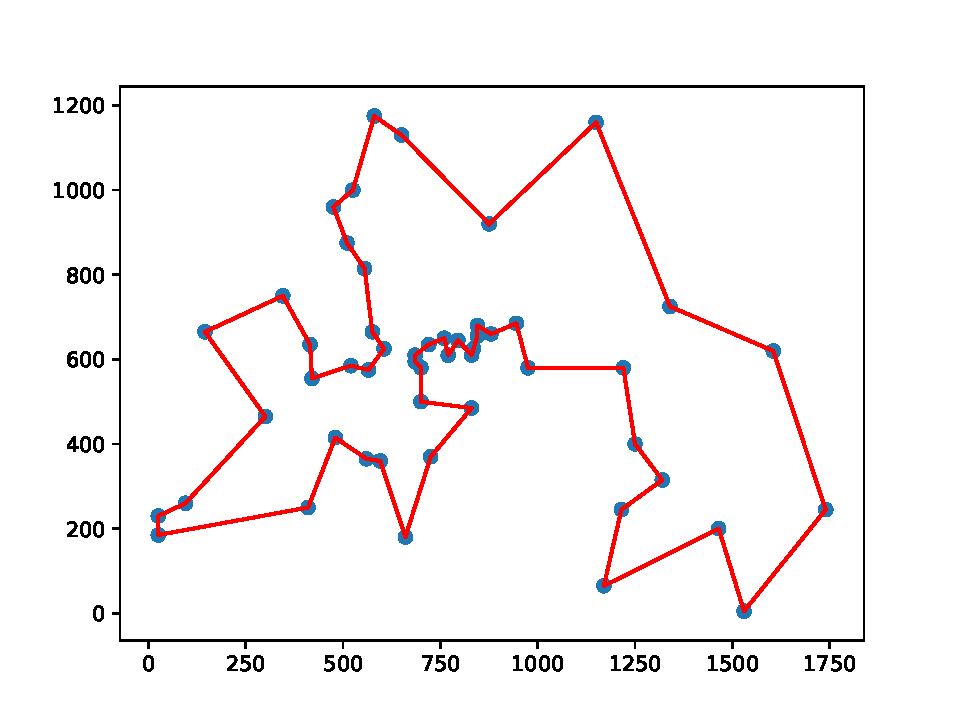
\includegraphics[width=\textwidth]{../Implementation/gen/best_path_gtspasms_berlin52}\\
			{\color{blue}GTSPA-SMS}
		\end{column}
	\end{columns}
	\begin{columns}
		\begin{column}{0.32\textwidth}
			\centering
			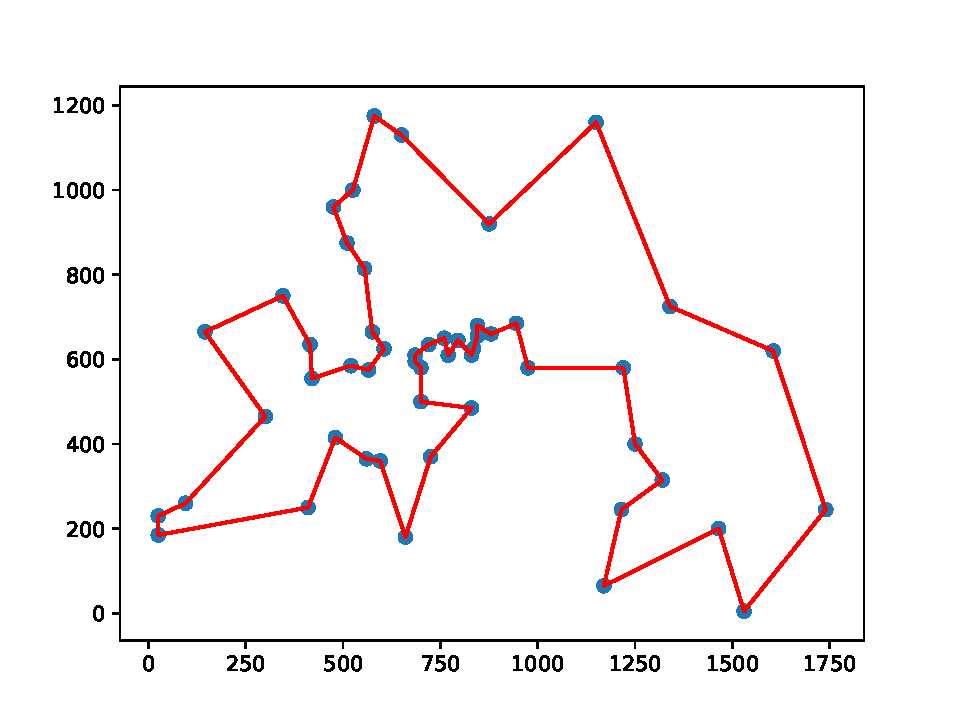
\includegraphics[width=\textwidth]{../Implementation/gen/best_path_gtspasm_berlin52}\\
			{\color{blue}GTSPA-SM}
		\end{column}
		\begin{column}{0.32\textwidth}
			\centering
			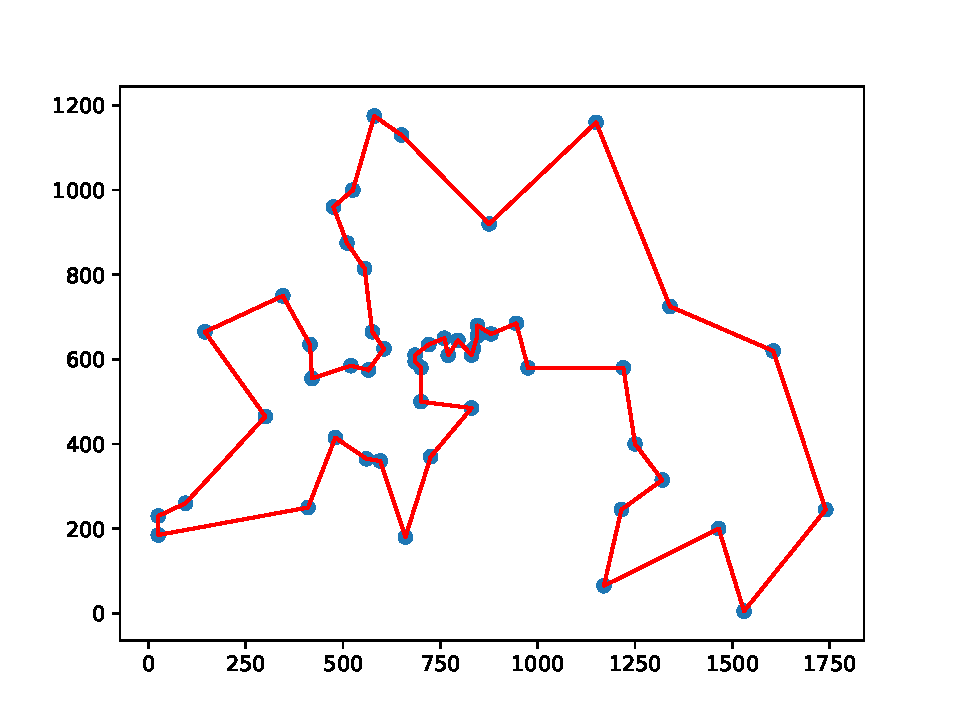
\includegraphics[width=\textwidth]{../Implementation/gen/optimal_path_berlin52}\\
			{\color{blue}Optimal}
		\end{column}
	\end{columns}
}

\frame[t]{
	\begin{columns}
		\begin{column}{0.32\textwidth}
			\centering
			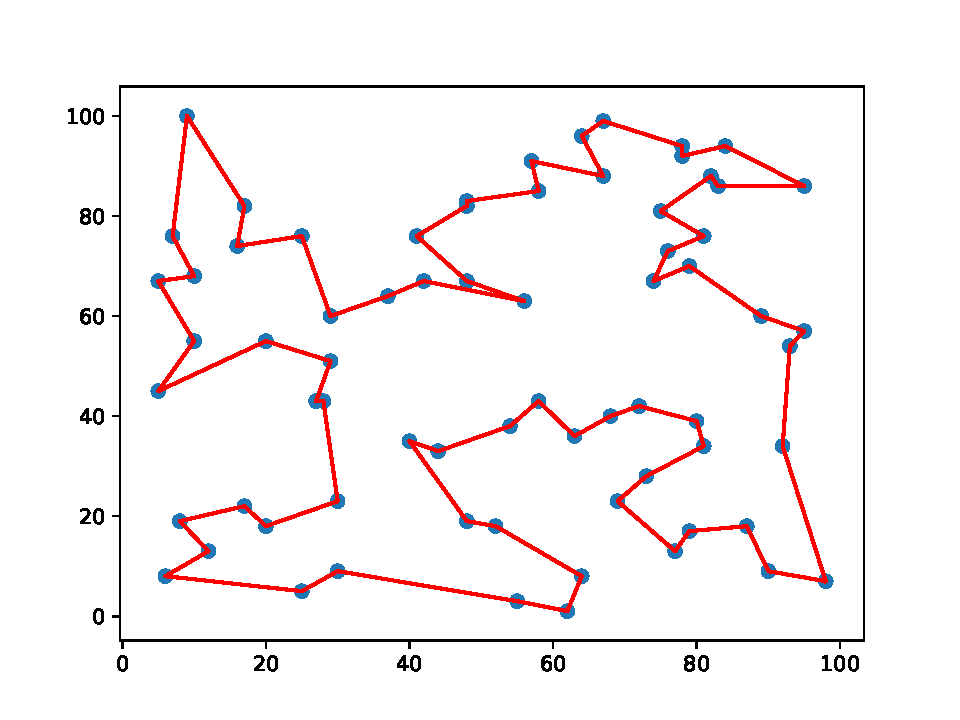
\includegraphics[width=\textwidth]{../Implementation/gen/best_path_dtsa_st70}\\
			{\color{blue}DTSA}
		\end{column}
		\begin{column}{0.32\textwidth}
			\centering
			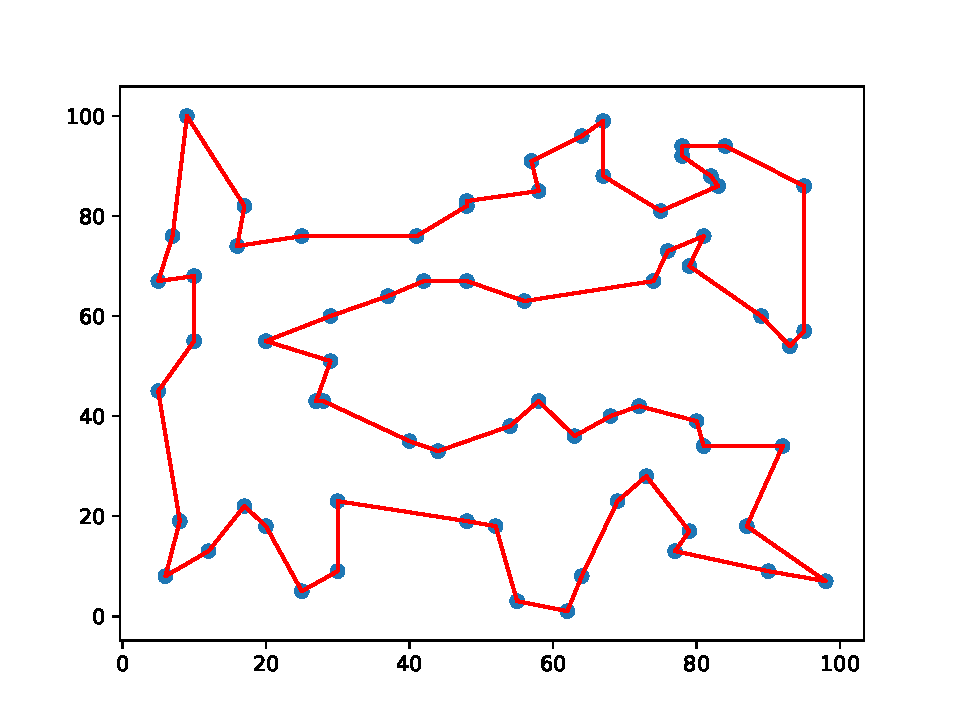
\includegraphics[width=\textwidth]{../Implementation/gen/best_path_gtspams_st70}\\
			{\color{blue}GTSPA-MS}
		\end{column}
		\begin{column}{0.32\textwidth}
			\centering
			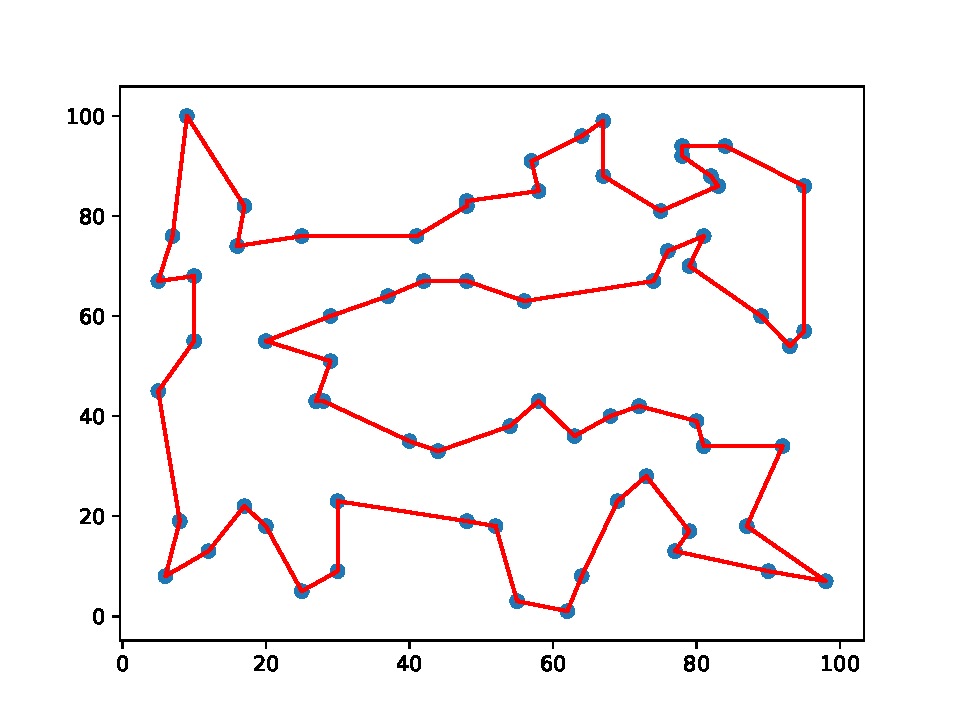
\includegraphics[width=\textwidth]{../Implementation/gen/best_path_gtspasms_st70}\\
			{\color{blue}GTSPA-SMS}
		\end{column}
	\end{columns}
	\begin{columns}
		\begin{column}{0.32\textwidth}
			\centering
			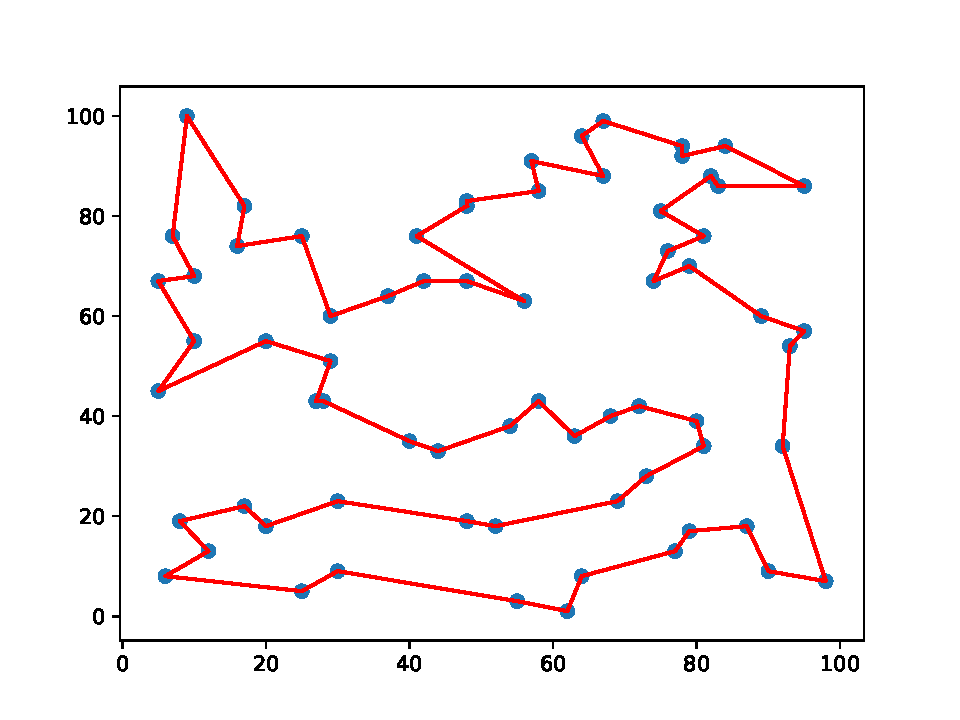
\includegraphics[width=\textwidth]{../Implementation/gen/best_path_gtspasm_st70}\\
			{\color{blue}GTSPA-SM}
		\end{column}
		\begin{column}{0.32\textwidth}
			\centering
			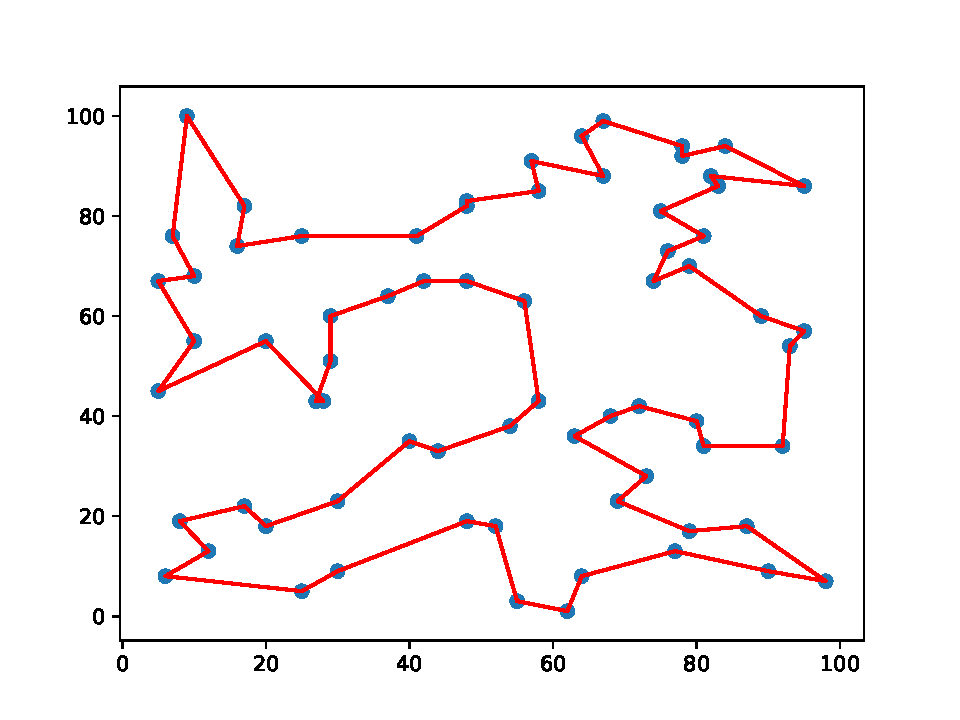
\includegraphics[width=\textwidth]{../Implementation/gen/optimal_path_st70}\\
			{\color{blue}Optimal}
		\end{column}
	\end{columns}
}

\frame[t]{
	\begin{columns}
		\begin{column}{0.32\textwidth}
			\centering
			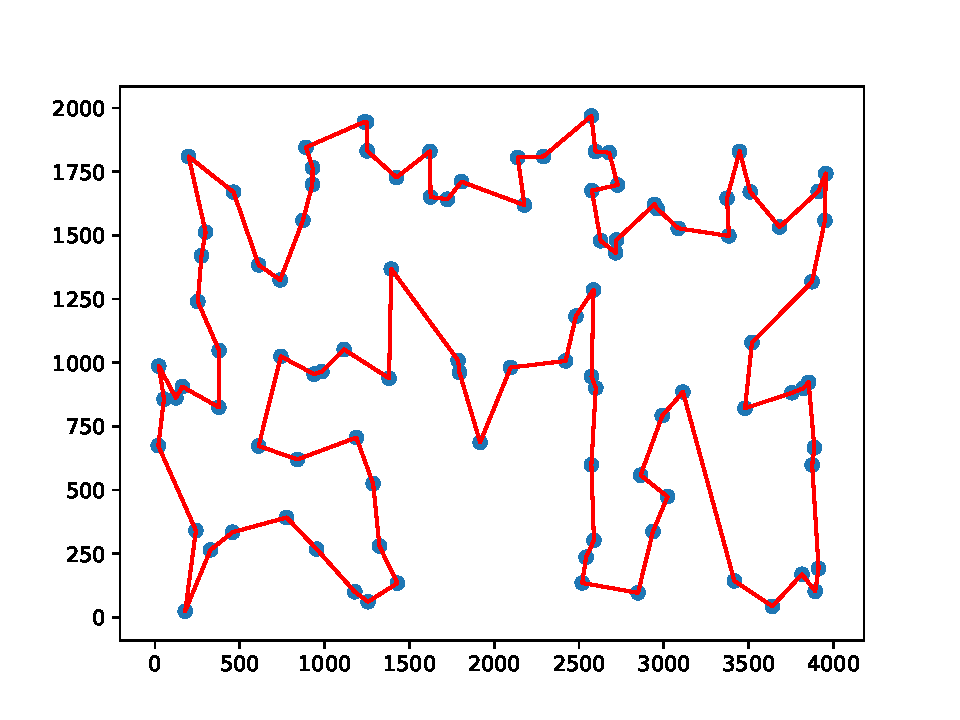
\includegraphics[width=\textwidth]{../Implementation/gen/best_path_dtsa_kroA100}\\
			{\color{blue}DTSA}
		\end{column}
		\begin{column}{0.32\textwidth}
			\centering
			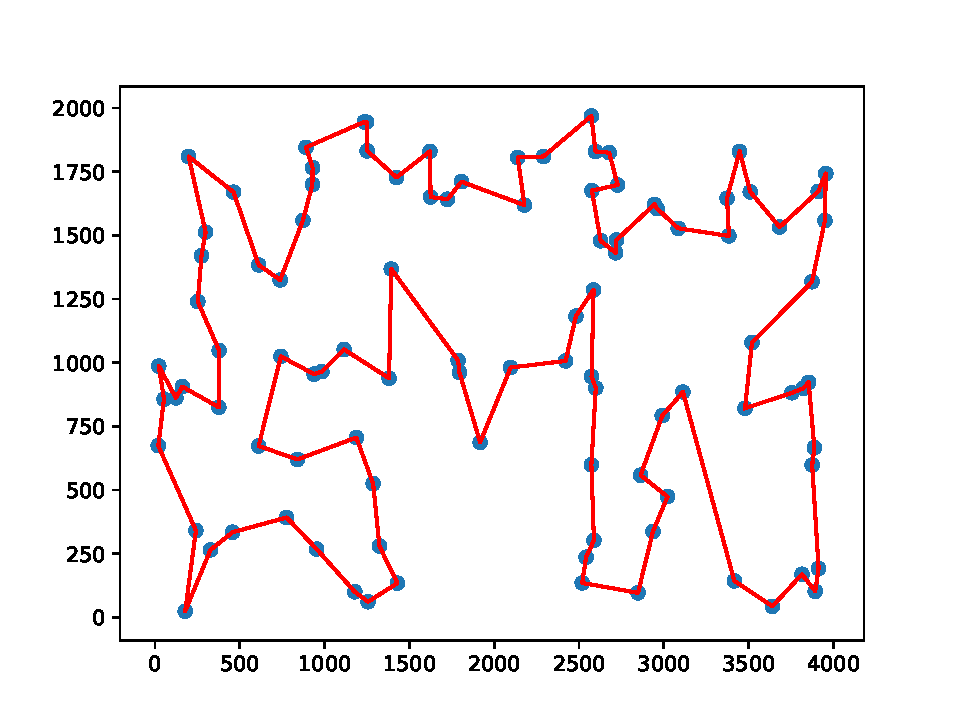
\includegraphics[width=\textwidth]{../Implementation/gen/best_path_gtspams_kroA100}\\
			{\color{blue}GTSPA-MS}
		\end{column}
		\begin{column}{0.32\textwidth}
			\centering
			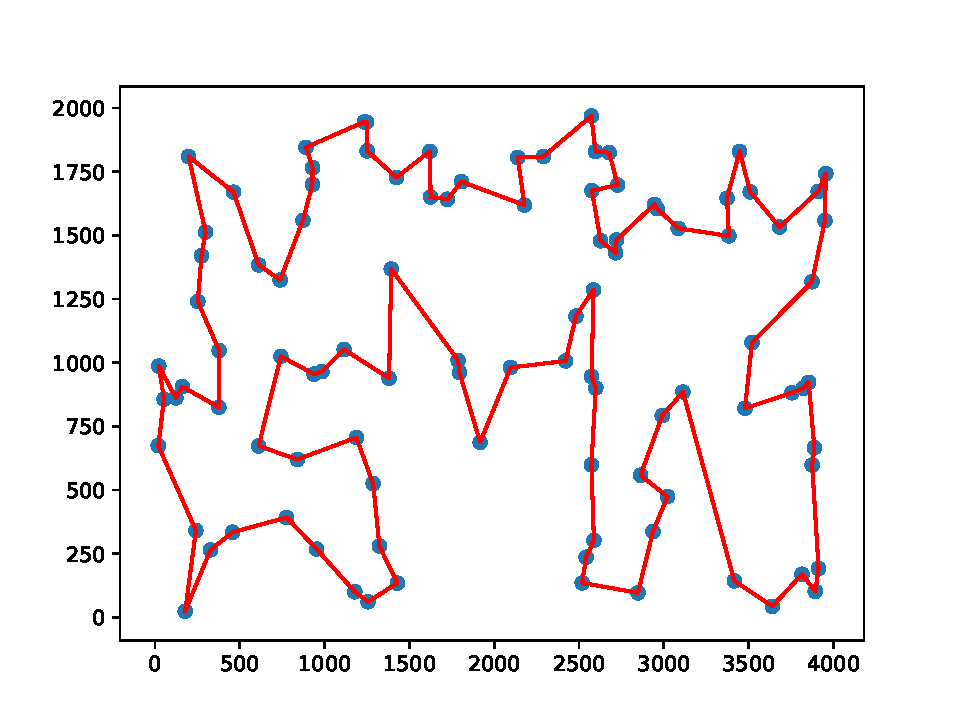
\includegraphics[width=\textwidth]{../Implementation/gen/best_path_gtspasms_kroA100}\\
			{\color{blue}GTSPA-SMS}
		\end{column}
	\end{columns}
	\begin{columns}
		\begin{column}{0.32\textwidth}
			\centering
			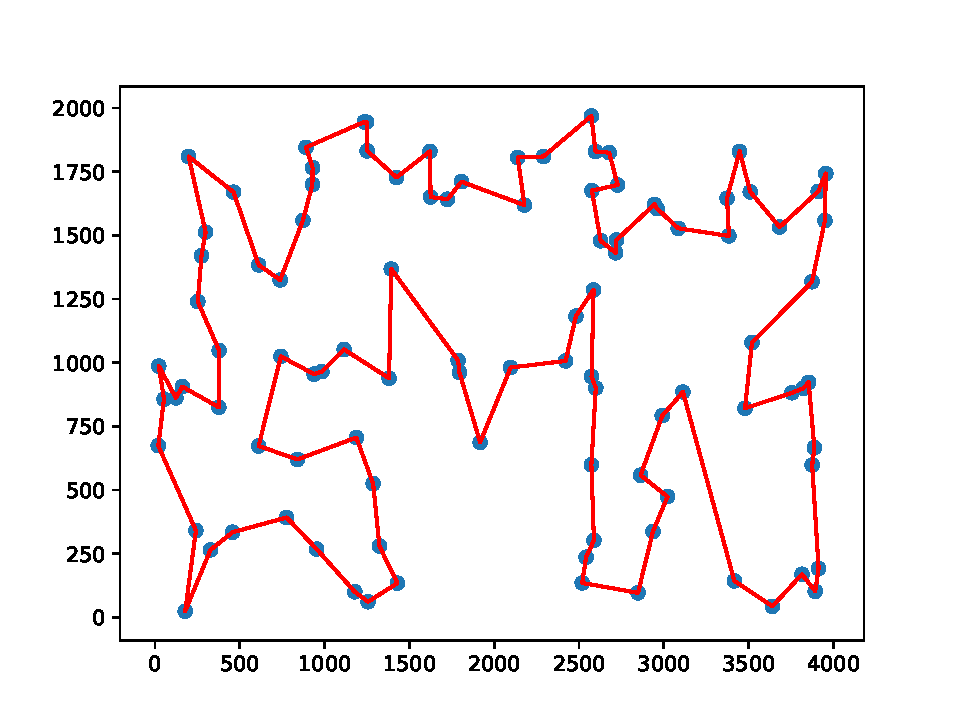
\includegraphics[width=\textwidth]{../Implementation/gen/best_path_gtspasm_kroA100}\\
			{\color{blue}GTSPA-SM}
		\end{column}
		\begin{column}{0.32\textwidth}
			\centering
			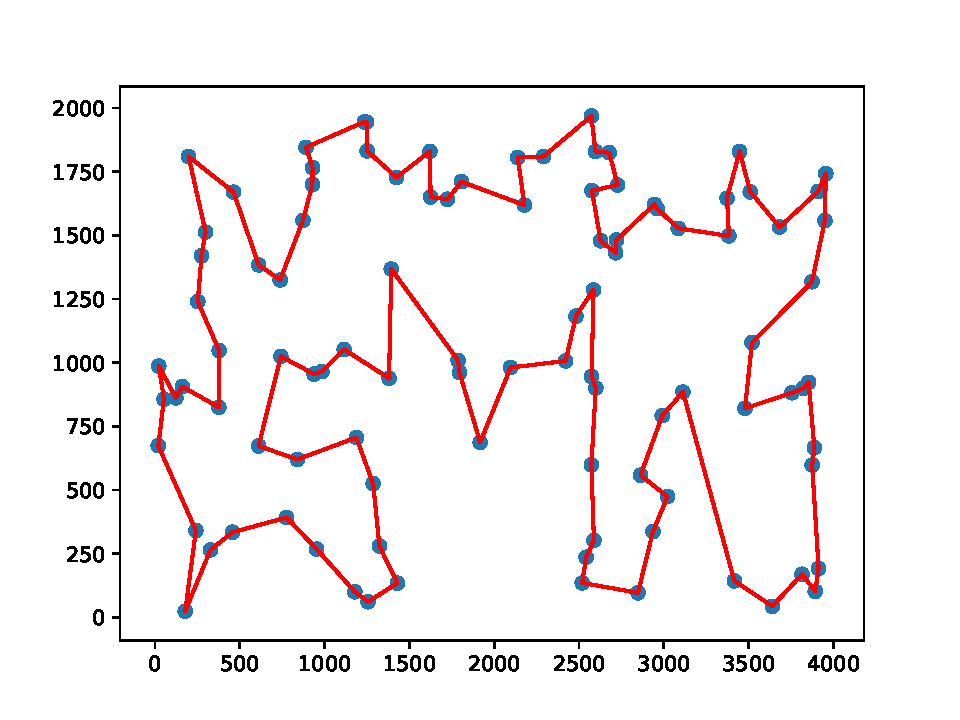
\includegraphics[width=\textwidth]{../Implementation/gen/optimal_path_kroA100}\\
			{\color{blue}Optimal}
		\end{column}
	\end{columns}
}

\frame[t]{
	\begin{columns}
		\begin{column}{0.32\textwidth}
			\centering
			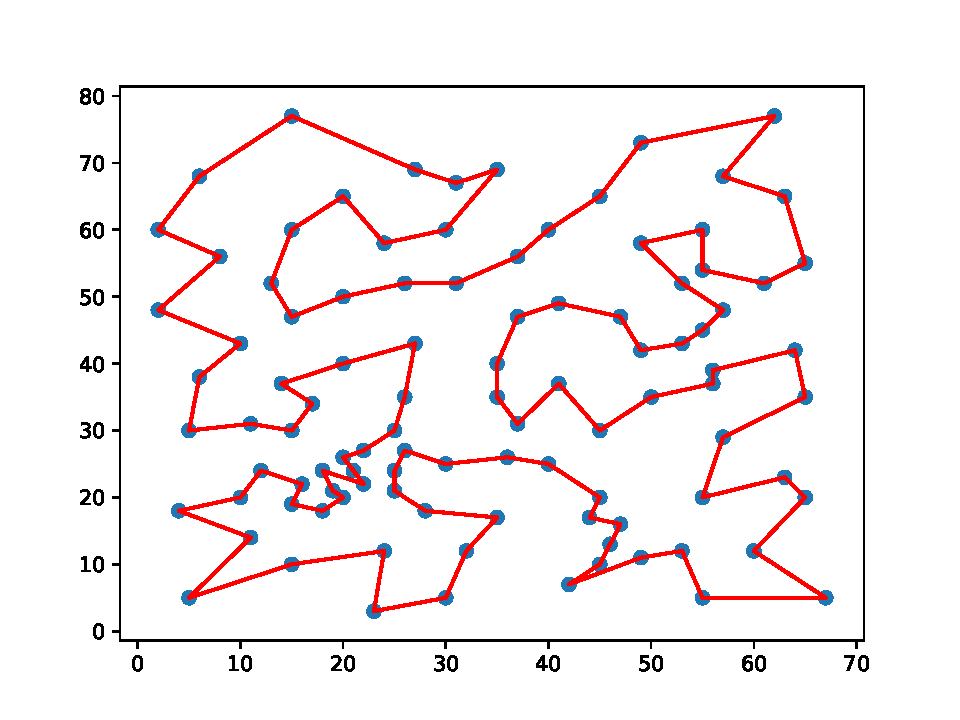
\includegraphics[width=\textwidth]{../Implementation/gen/best_path_dtsa_eil101}\\
			{\color{blue}DTSA}
		\end{column}
		\begin{column}{0.32\textwidth}
			\centering
			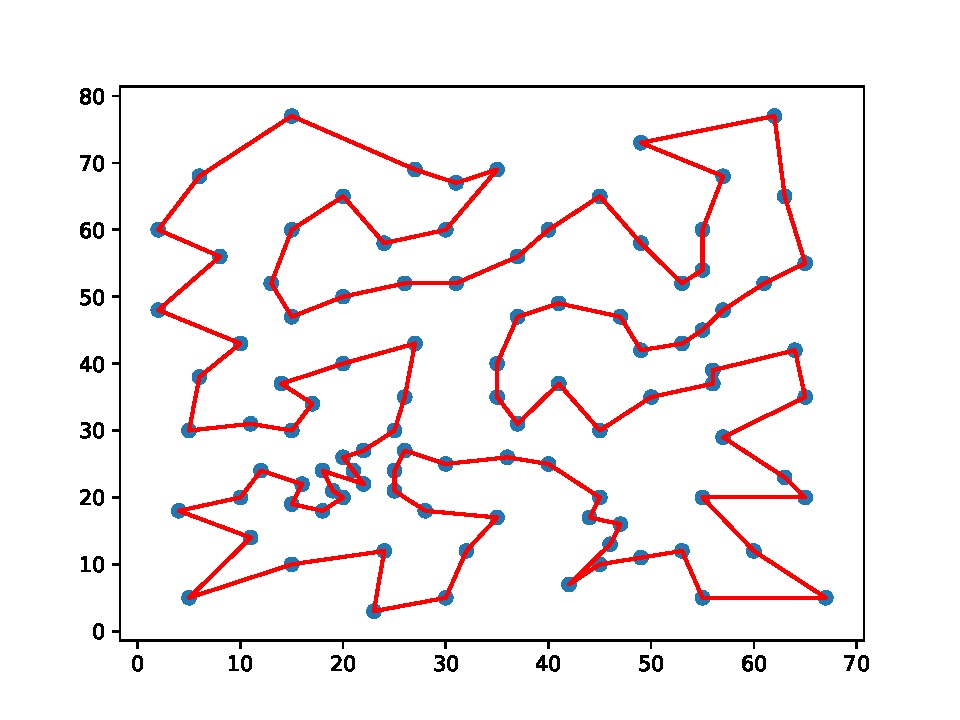
\includegraphics[width=\textwidth]{../Implementation/gen/best_path_gtspams_eil101}\\
			{\color{blue}GTSPA-MS}
		\end{column}
		\begin{column}{0.32\textwidth}
			\centering
			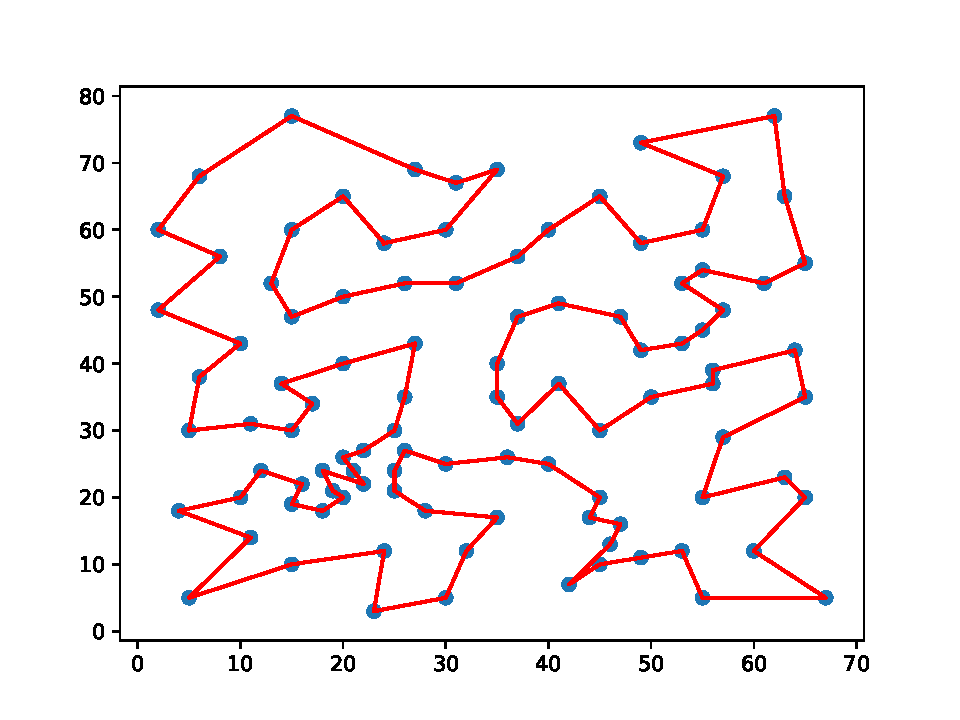
\includegraphics[width=\textwidth]{../Implementation/gen/best_path_gtspasms_eil101}\\
			{\color{blue}GTSPA-SMS}
		\end{column}
	\end{columns}
	\begin{columns}
		\begin{column}{0.32\textwidth}
			\centering
			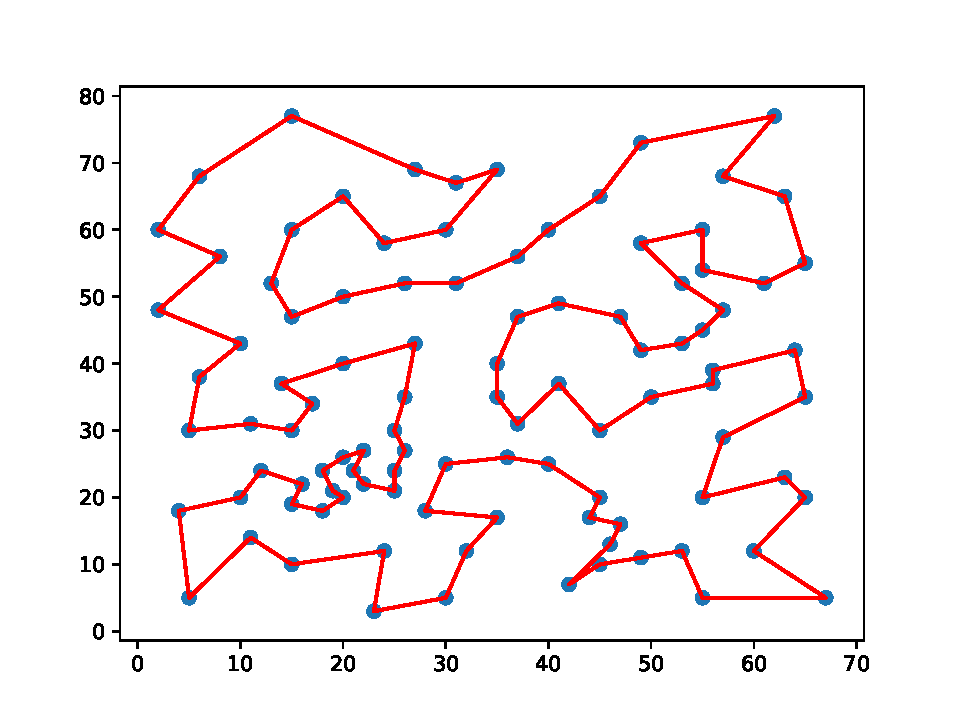
\includegraphics[width=\textwidth]{../Implementation/gen/best_path_gtspasm_eil101}\\
			{\color{blue}GTSPA-SM}
		\end{column}
		\begin{column}{0.32\textwidth}
			\centering
			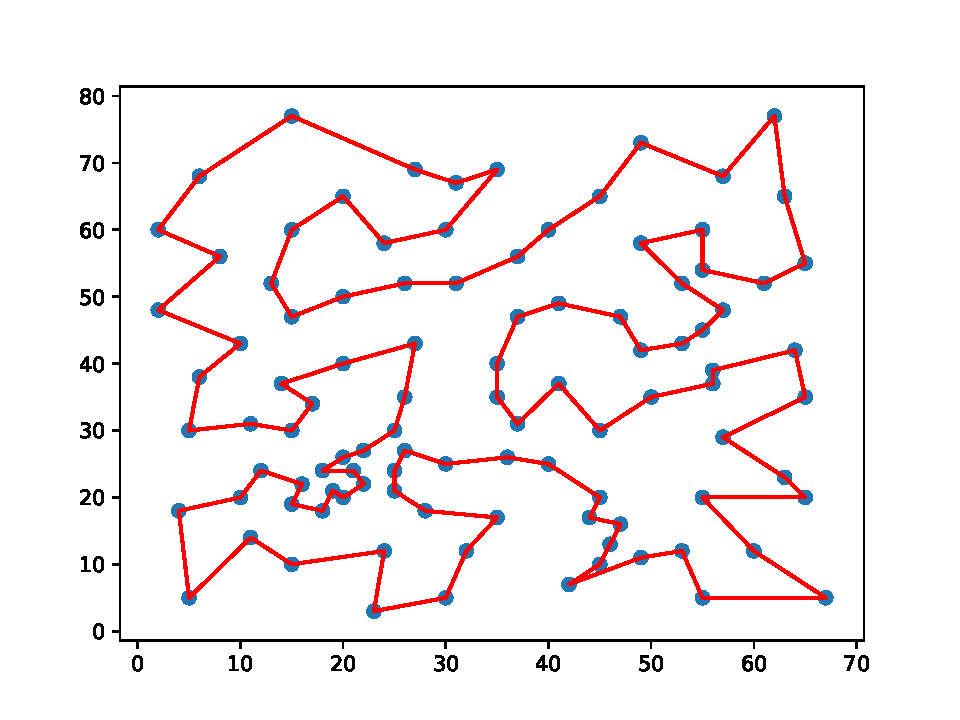
\includegraphics[width=\textwidth]{../Implementation/gen/optimal_path_eil101}\\
			{\color{blue}Optimal}
		\end{column}
	\end{columns}
}

\frame[t]{
	\begin{columns}
		\begin{column}{0.32\textwidth}
			\centering
			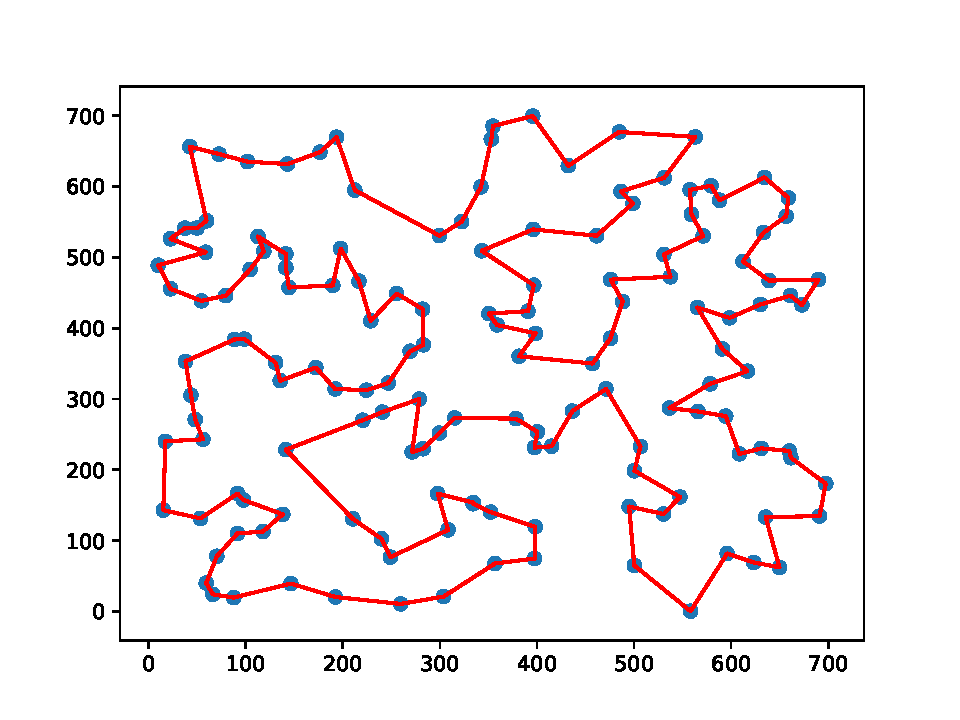
\includegraphics[width=\textwidth]{../Implementation/gen/best_path_dtsa_ch150}\\
			{\color{blue}DTSA}
		\end{column}
		\begin{column}{0.32\textwidth}
			\centering
			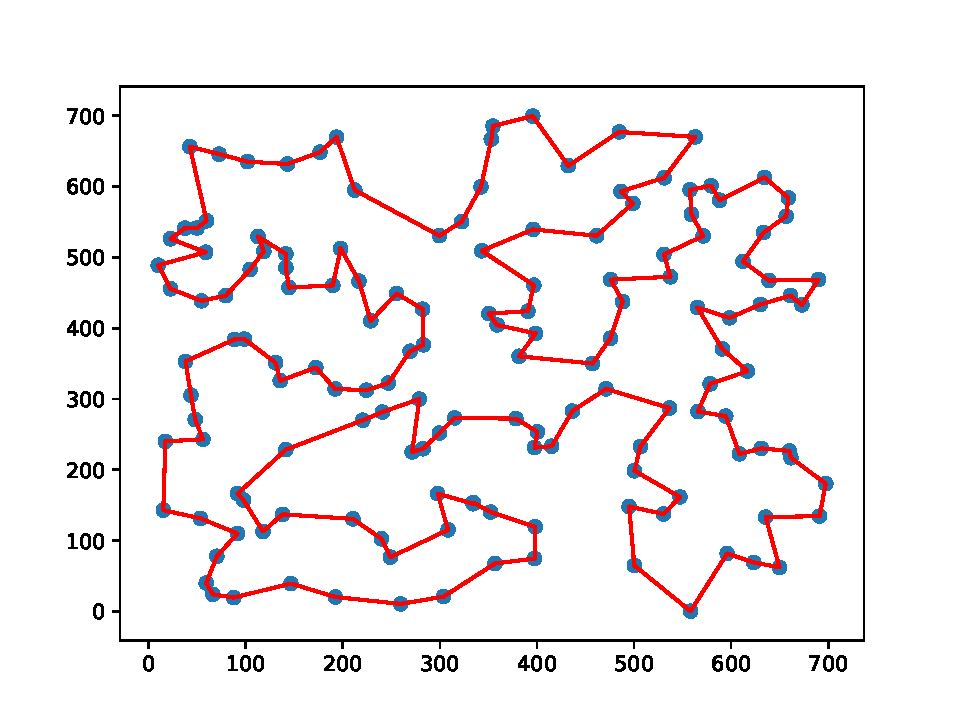
\includegraphics[width=\textwidth]{../Implementation/gen/best_path_gtspams_ch150}\\
			{\color{blue}GTSPA-MS}
		\end{column}
		\begin{column}{0.32\textwidth}
			\centering
			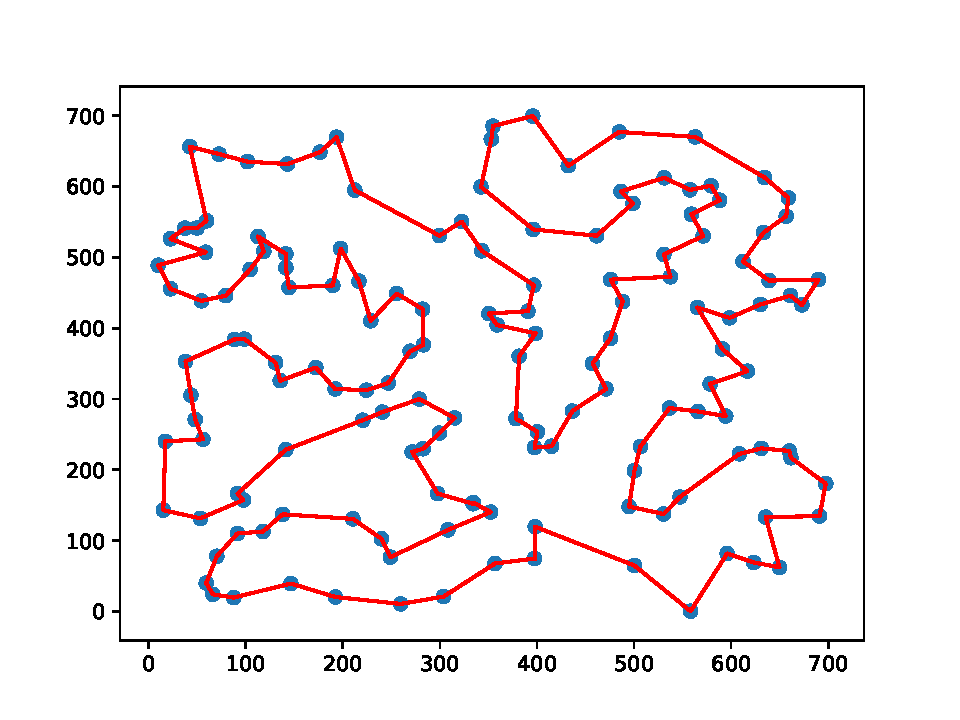
\includegraphics[width=\textwidth]{../Implementation/gen/best_path_gtspasms_ch150}\\
			{\color{blue}GTSPA-SMS}
		\end{column}
	\end{columns}
	\begin{columns}
		\begin{column}{0.32\textwidth}
			\centering
			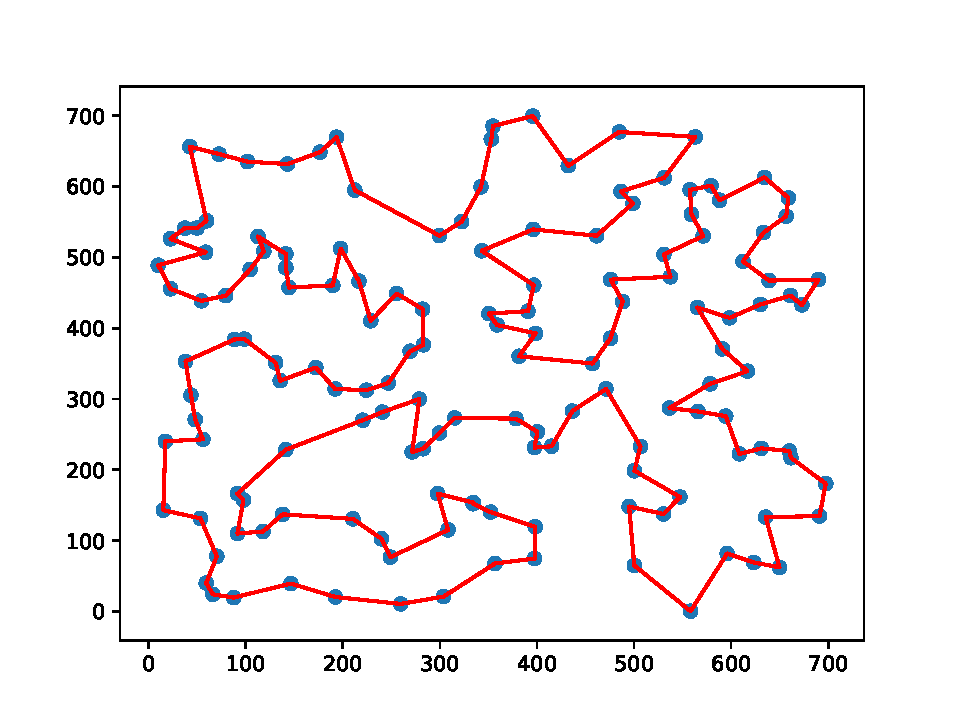
\includegraphics[width=\textwidth]{../Implementation/gen/best_path_gtspasm_ch150}\\
			{\color{blue}GTSPA-SM}
		\end{column}
		\begin{column}{0.32\textwidth}
			\centering
			\includegraphics[width=\textwidth]{../Implementation/gen/optimal_path_ch150}\\
			{\color{blue}Optimal}
		\end{column}
	\end{columns}
}

\end{document}